\section{Unified Predictive Motion Planning via a Constant
State-Transition Double-Integrator
Backbone}\label{unified-predictive-motion-planning-via-a-constant-state-transition-double-integrator-backbone}

\begin{center}\rule{0.5\linewidth}{0.5pt}\end{center}

\subsection{Abstract}\label{abstract}

Traditional robotic motion planning separates geometric path-finding
from temporal parameterization, limiting a robot's ability to react to
dynamic obstacles without costly replanning loops. This paper presents a
unified, real-time local Predictive Motion Planner formulated directly
in the time domain, building on a two-layer architecture previously
demonstrated for physical human--robot interaction (pHRI) compliance.
The central observation is that a virtual double-integrator planner
yields a constant state-transition matrix \(A_d\) independent of robot
configuration. Consequently, the dynamics prediction matrices can be
precomputed offline, reducing online planning to a small convex
Quadratic Program (QP) with fixed dynamics structure. The decoupled
box-constrained case runs comfortably at 100 Hz or higher; coupled
obstacle rows remain convex and achieve 100 Hz p95 timing in the Python
harness with fixed-sparsity updates, although worst-case cycles can
exceed 10 ms without further implementation optimization.

Layer 1 maps the multi-variable joint space into a set of
configuration-independent double-integrator prediction models. Layer 2
solves the convex QP at high frequency, simultaneously enforcing
kinematic limits (velocity, acceleration) and linearized obstacle
constraints. The framework delivers smooth, continuous position/velocity
profiles \((q_d, \dot{q}_d)\) with hard-bounded, piecewise-constant
acceleration \(\ddot{q}_d\), and demonstrates bounded-latency reactive
deflection in cluttered spaces without structural replanning downtime.
When continuous acceleration is required, the same nilpotent-structure
argument extends to a piecewise-jerk triple-integrator backbone. The
constant-\(A_d\) structure enables bounded per-cycle reaction latency
that is structurally unavailable to batch planning pipelines.

\begin{center}\rule{0.5\linewidth}{0.5pt}\end{center}

\subsection{I. Introduction}\label{i.-introduction}

Modern robotic systems deployed in unstructured or human-shared
environments must track planned trajectories with high precision while
remaining responsive to dynamic workspace changes. Classical motion
planning pipelines address these demands sequentially. A geometric
planner (e.g., OMPL {[}1{]}) first searches for a collision-free path in
configuration space. A separate time-parameterization stage (e.g.,
Time-Optimal Trajectory Generation, TOTG {[}2{]}) then maps this spatial
path into a timed trajectory via a transformation \(s \rightarrow t\)
from arc-length to time. This decoupling introduces a fundamental
limitation: if an obstacle shifts or a human interjects during
execution, the entire pipeline must be interrupted for a full re-plan,
incurring latency that is incompatible with real-time reactive behavior.

Recent work on predictive impedance control for pHRI has demonstrated
that a two-layer architecture grounded in a configuration-independent
double-integrator model can yield sub-millisecond QP solves while
strictly enforcing actuator constraints {[}3{]}. The key structural
insight is that the residual plant reduces to a linear system whose
state-transition matrix \(A_d\) is constant across all configurations.
This enables the free-response prediction matrix \(\Phi\) to be
precomputed entirely offline, leaving only lightweight matrix--vector
operations at runtime.

\textbf{The central observation of this paper is that a virtual
double-integrator planner yields a constant state-transition matrix
independent of robot configuration. Consequently, all dynamics
prediction matrices can be precomputed offline, reducing online planning
to a small convex QP with fixed dynamics structure.} This paper pivots
the pHRI architectural principle into a unified time-domain Predictive
Motion Planner. Rather than inventing a new planning paradigm, we show
that a previously developed pHRI MPC architecture naturally yields an
efficient predictive local motion planner with bounded-latency obstacle
avoidance when applied in a purely software-defined planning context.

The resulting framework should be understood as a \textbf{local
predictive motion planner (receding-horizon trajectory optimizer)}
rather than a complete global planner. It does not perform global
search; obstacle avoidance is local and relies on linearization and
artificial potential fields. The framework's distinctive properties are:

\begin{itemize}
\tightlist
\item
  Bounded by a fixed optimization structure whose size grows with the
  number of active obstacle constraints.
\item
  Simultaneous enforcement of kinematic limits and obstacle constraints
\item
  No spatial-to-temporal transformation stage
\item
  Offline precomputation of all dynamics prediction matrices via the
  constant-\(A_d\) property
\item
  Smooth \(C^1\) output with hard-bounded acceleration; optional
  piecewise-jerk extension for continuous acceleration
\end{itemize}

The paper is organized as follows. Section II presents the mathematical
backbone. Section III describes the receding-horizon QP formulation.
Section IV details two complementary obstacle avoidance strategies.
Section V analyzes key architectural properties. Section VI reports
experimental benchmarks. Sections VII--IX present implementation notes,
discussion, and conclusions.

\begin{center}\rule{0.5\linewidth}{0.5pt}\end{center}

\subsection{II. Mathematical Framework and System
Structure}\label{ii.-mathematical-framework-and-system-structure}

The objective of motion planning is to construct a feasible trajectory
that drives the robot through a sequence of task-space or joint-space
waypoints while satisfying kinematic and environmental constraints.
Unlike motion control, which computes actuator commands for a physical
plant, motion planning operates at the trajectory level and produces a
reference trajectory for a downstream controller.

Let the robot configuration be \(q \in \mathbb{R}^n\) and let the
task-space position be determined by the forward kinematics

\[
p=f(q).
\]

The planning problem is to generate a trajectory

\[
q(t),\dot q(t),\ddot q(t)
\]

that satisfies waypoint requirements, joint limits, velocity limits,
acceleration limits, and obstacle-avoidance constraints.

To parameterize the admissible trajectory space, the planner employs a
configuration-independent double-integrator backbone. This backbone may
be interpreted either as (i) the residual system obtained after
feedforward cancellation of robot dynamics, as in the pHRI architecture,
or (ii) a virtual trajectory-generation model used solely for planning.
In both interpretations the resulting state-transition matrix is
identical and constant.

\[
\ddot q_i=u_i.
\]

The double-integrator backbone is not used to model actuator-level
dynamics during planning. Instead, it serves as a trajectory-generation
backbone whose state consists of planned joint positions and velocities,
and whose outputs are reference trajectories for a downstream tracking
controller. The optimization is therefore performed over a family of
kinematically feasible trajectories rather than over actuator commands.

The double-integrator parameterization is attractive because it
guarantees continuous position and velocity trajectories while allowing
acceleration limits to be enforced directly as linear constraints.
Furthermore, the resulting state-transition matrix is configuration
independent, enabling all dynamics prediction matrices to be precomputed
offline.

\subsubsection{A. Double-Integrator Backbone from Dynamic
Cancellation}\label{a.-double-integrator-backbone-from-dynamic-cancellation}

Consider the standard rigid-body manipulator dynamics

\[ M(q)\ddot q + C(q,\dot q)\dot q + g(q)=\tau . \]

In the dynamic-cancellation interpretation, the planner operates on
joint coordinates parameterized by a double-integrator backbone.
Following the two-layer architecture previously developed for pHRI, a
feedforward compensation term is used to cancel the
configuration-dependent nonlinear dynamics. The control input is
decomposed as

\[ \tau = M(q)u + C(q,\dot q)\dot q + g(q), \]

where \(u\) is a virtual acceleration command generated by the
predictive layer. Substituting into the manipulator dynamics yields

\[ \ddot q = u. \]

Defining the state
\(x = \begin{bmatrix} q ^\top, \dot q ^\top \end{bmatrix} ^\top\), the
residual system becomes

\[\dot x = \begin{bmatrix} 0&I\\ 0&0 \end{bmatrix}x +
\begin{bmatrix} 0\\ I \end{bmatrix}u, \]

which is a configuration-independent double integrator.

The key consequence is that the system matrix is constant and nilpotent.
After discretization, the planning-model state-transition matrix \(A_d\)
is independent of robot configuration and operating point. Therefore the
dynamics prediction matrices required by the receding-horizon optimizer
can be computed once offline and reused unchanged throughout execution.

This double-integrator backbone is identical to that used in the pHRI
Impedance MPC architecture; the difference is that the present work
employs it for predictive motion planning rather than
disturbance-rejecting impedance regulation.

\subsubsection{\texorpdfstring{B. Exact ZOH Discretization and the
Constant \(A_d\)
Property}{B. Exact ZOH Discretization and the Constant A\_d Property}}\label{b.-exact-zoh-discretization-and-the-constant-a_d-property}

The continuous system matrix \(A_c\) is nilpotent: \(A_c^2 = 0\).
Consequently, for a planning period \(\Delta t\), the matrix exponential
truncates exactly:

\[e^{A_c \Delta t} = I + A_c \Delta t\]

and the exact Zero-Order Hold (ZOH) discretization yields:

\[A_d = \begin{bmatrix} 1 & \Delta t \\ 0 & 1 \end{bmatrix}, \qquad B_d = \begin{bmatrix} \frac{\Delta t^2}{2} \\ \Delta t \end{bmatrix}\]

The critical structural result is that \(A_d\) is \textbf{constant and
identical for every joint at every configuration}. This stands in sharp
contrast to physical plant discretizations (e.g., from linearized
manipulator dynamics), where \(A_d\) depends on \(M(q)\),
\(C(q,\dot{q})\), and Jacobian terms that vary continuously with robot
state.

Since \(A_d\) is invariant, the trajectory prediction matrices over a
finite horizon \(N\):

\[\Phi = \begin{bmatrix} A_d \\ A_d^2 \\ \vdots \\ A_d^N \end{bmatrix}, \qquad \Gamma = \begin{bmatrix} B_d & 0 & \cdots & 0 \\ A_d B_d & B_d & \cdots & 0 \\ \vdots & & \ddots & \vdots \\ A_d^{N-1} B_d & \cdots & A_d B_d & B_d \end{bmatrix}\]

can be \textbf{precomputed entirely offline and stored as constants}. At
runtime, trajectory rollouts over the horizon reduce to a single
matrix--vector multiply, enabling high-frequency planning loops. This is
the enabling structural insight: the computational burden of trajectory
prediction is fully decoupled from robot configuration.

\begin{center}\rule{0.5\linewidth}{0.5pt}\end{center}

\subsection{III. Receding-Horizon Optimization (Layer 2 QP
Planner)}\label{iii.-receding-horizon-optimization-layer-2-qp-planner}

\subsubsection{A. Optimization Problem
Structure}\label{a.-optimization-problem-structure}

At each planning time step, the planner solves for the optimal
acceleration profile sequence across the prediction horizon:

\[U = \begin{bmatrix} u(0) \\ u(1) \\ \vdots \\ u(N-1) \end{bmatrix} \in \mathbb{R}^{nN}\]

where \(n\) is the number of joints and \(N\) is the horizon length
(e.g., \(nN = 7\times 20 = 140\) decision variables for the 7-DOF FR3
with \(N=20\)). The predicted state trajectory is:

\[X = \Phi x(k) + \Gamma U\]

which is affine in \(U\) given the current planner state \(x(k)\). This
linearity makes all downstream constraints (kinematic bounds, obstacle
avoidance) convex in the decision variable. Absent obstacle coupling,
the Hessian is block-diagonal and the problem separates into \(n\)
independent per-joint QPs of size \(N\).

\subsubsection{B. Cost Function: Tracking and
Smoothness}\label{b.-cost-function-tracking-and-smoothness}

The objective function minimizes the weighted sum of tracking deviations
from a goal state \(x_{\text{goal}} = [q_{\text{goal}}, 0]^\top\) and
control effort. We write the stage cost with the conventional
\(\tfrac{1}{2}\) scaling,

\[J(U)=\frac{1}{2}\left(\Phi x(k)+\Gamma U-\mathbf{1}_N\otimes x_{\text{goal}}\right)^\top
\bar Q\left(\Phi x(k)+\Gamma U-\mathbf{1}_N\otimes x_{\text{goal}}\right)
+\frac{1}{2}U^\top\bar R U,\]

so that collecting the terms depending on \(U\) gives

\[\min_{U} \; \frac{1}{2} U^\top H U + h^\top U\]

where:

\[H = \Gamma^\top \bar{Q} \Gamma + \bar{R}, \qquad h = \Gamma^\top \bar{Q} \, x_{\text{free,err}}\]

and
\(x_{\text{free,err}} = \Phi x(k) - \mathbf{1}_N \otimes x_{\text{goal}}\)
is the unforced deviation from the goal. Equivalently, if the same
least-squares cost is written without the leading \(\tfrac{1}{2}\)
factors, both \(H\) and \(h\) are multiplied by \(2\); the optimizer is
unchanged because this scales the entire objective by a positive
constant. All OSQP calls use the convention above. The remaining
definitions are: - the full goal state
\(x_{\text{goal}}=[q_{\text{goal}},0]^\top\) replicated across all \(N\)
horizon steps, - stage weights \(Q = \text{blkdiag}(K_q, D_q)\)
penalizing position and velocity errors, - control cost matrix \(R\)
penalizing large accelerations to regularize the trajectory, - terminal
weight \(Q_f = \gamma Q\) (with \(\gamma \approx 5\)--\(10\)) applied at
the final horizon step to encourage convergence, - horizon-stacked
weights \(\bar Q = \mathrm{blkdiag}(Q,\dots,Q,Q_f)\) and
\(\bar R = I_N \otimes R\).

Because \(H\) is the sum of a positive semi-definite matrix (from
\(\bar{Q}\)) and a positive definite matrix (from \(\bar{R}\) with
\(R \succ 0\)), the QP is \textbf{strictly convex} for all
configurations and all time steps. A unique global minimizer exists and
is found efficiently by operator-splitting solvers such as OSQP {[}4{]}
with warm-starting, typically converging in under 0.5 ms.

\textbf{Weight tuning guidance.} The weights have intuitive roles that
make initial tuning straightforward. \(K_q\) (position error weight)
sets convergence aggressiveness: increasing it pulls the planner toward
the goal faster but risks saturating the acceleration limit. \(D_q\)
(velocity error weight) provides damping and prevents overshoot; a good
starting ratio is \(D_q \approx 2\sqrt{K_q}\) (critically-damped
second-order response). \(R\) (acceleration regularization) trades
smoothness against speed: larger \(R\) produces gentler profiles but
increases time-to-goal. The terminal multiplier \(\gamma\) compensates
for the finite horizon; \(\gamma = 5\)--\(10\) is sufficient for
\(N \geq 20\). For the FR3 experiments reported here, the values used
are \(K_q = 100\), \(D_q = 20\), \(R = 0.1\,I\), \(\gamma = 8\) (all
per-joint, scalar). A practical tuning sequence is: (1) set \(R\) small
and increase \(K_q\) until the planner reaches goals comfortably within
kinematic limits; (2) increase \(D_q\) until overshoot disappears; (3)
increase \(R\) if the resulting jerk is unacceptable for the
application.

\subsubsection{C. Kinematic Hard
Constraints}\label{c.-kinematic-hard-constraints}

Physical joint limits are enforced as hard inequality constraints on the
predicted state and input sequences. For each joint \(i\) and each step
\(k\) along the horizon:

\textbf{Velocity bounds:}
\[-\dot{q}_{i,\max} \leq \dot{q}_{i}(k) \leq \dot{q}_{i,\max} \quad \forall k \in \{1,\dots,N\}\]

\textbf{Acceleration (input) bounds:}
\[-u_{i,\max} \leq u_i(k) \leq u_{i,\max} \quad \forall k \in \{0,\dots,N-1\}\]

Since the predicted states are affine in \(U\) (via \(\Gamma\)), these
constraints translate to a set of linear inequalities
\(C_{\text{kin}} U \leq d_{\text{kin}}\) assembled once from the
precomputed \(\Gamma\) matrix and fixed online. Optionally, joint
position limits \(q_{i,\min} \leq q_i(k) \leq q_{i,\max}\) can be
appended with no additional computational overhead.

\begin{center}\rule{0.5\linewidth}{0.5pt}\end{center}

\subsection{IV. Incorporating Workspace Obstacle
Avoidance}\label{iv.-incorporating-workspace-obstacle-avoidance}

The linearity of the predicted joint positions with respect to \(U\)
makes it straightforward to incorporate obstacle avoidance constraints
without breaking convexity. Two complementary methods are presented.

\subsubsection{A. Convex Corridor Polytope Constraints (Hard
Constraints)}\label{a.-convex-corridor-polytope-constraints-hard-constraints}

Cartesian obstacles detected by perception systems are represented as
half-space inequalities in task space:

\[A_{\text{obs}} \, p(k) \leq b_{\text{obs}}\]

where \(p(k) \in \mathbb{R}^3\) is the predicted end-effector (or link)
position at step \(k\). Using the robot's forward kinematics linearized
at the current operating point via the translational Jacobian
\(J_v(q_0)\):

\[p(k) \approx p_0 + J_v(q_0)\bigl(q(k) - q_0\bigr)\]

the workspace constraint becomes:

\[A_{\text{obs}} J_v(q_0) \, \Delta q(k) \leq b_{\text{obs}} - A_{\text{obs}} p_0\]

where \(\Delta q(k) = q(k) - q_0\) is linear in \(U\) through
\(\Gamma\). To make the QP row explicit, let \(E_{q,k}\) select the
predicted joint-position block at horizon step \(k\), so

\[q(k)=E_{q,k}\bigl(\Phi x(k_0)+\Gamma U\bigr).\]

Then each obstacle row has the affine form

\[
\underbrace{A_{\text{obs}}J_v(q_0)E_{q,k}\Gamma}_{C_{\text{obs},k}}\,U
\le
\underbrace{b_{\text{obs}}-A_{\text{obs}}p_0
-A_{\text{obs}}J_v(q_0)\bigl(E_{q,k}\Phi x(k_0)-q_0\bigr)}_{d_{\text{obs},k}} .
\]

Thus the free-response term is absorbed into the right-hand side, and
the obstacle constraint becomes a set of affine inequalities in \(U\),
fully compatible with the convex QP structure.

\textbf{Approximation quality.} Because \(J_v(q_0)\) is held constant
over the horizon rollout within a cycle, these rows form a first-order
local approximation of the safe corridor: exact near \(q_0\), but
increasingly inaccurate as the predicted motion leaves a neighborhood of
\(q_0\). This linearization is not automatically conservative. To obtain
a conservative half-space, each obstacle row should be tightened by a
bound on the forward-kinematics linearization error. The approximation
is refreshed by re-linearizing every cycle. A theoretical upper bound
follows from the second-order Taylor remainder: letting \(H_p(q_0)\)
denote the position Hessian (the tensor of second partial derivatives of
\(p\) with respect to \(q\), evaluated at \(q_0\)), the true
end-effector position satisfies

\[\|p(q) - (p_0 + J_v(q_0)\Delta q)\| \leq \tfrac{1}{2} \|H_p(q_0)\|_F \|\Delta q\|^2\]

where \(\|\cdot\|_F\) is the Frobenius norm. For an obstacle half-space
row \(a^\top p\le b\), a conservative tightened row is

\[a^\top\bigl(p_0+J_v(q_0)\Delta q(k)\bigr)\le b-\|a\|\,\varepsilon_p,\]

with
\(\varepsilon_p \geq \tfrac{1}{2}\|H_p\|_{F}\|\Delta q_{\max}\|^2\). The
position Hessian norm \(\|H_p\|_F\) was computed numerically for the FR3
by central-difference differentiation of the Jacobian at 5000
configurations sampled uniformly from the joint range; the resulting
distribution has mean \(0.91\) m/rad² and 95th-percentile \(1.43\)
m/rad², giving the range \(\approx 0.5\)--\(1.5\) m/rad² quoted below.
The accompanying harness reports representative end-horizon
linearization errors of 7.1 mm at 25\% joint speed over 0.1 s, 28.0 mm
at 25\% over 0.2 s, 28.0 mm at 50\% over 0.1 s, 106.4 mm at 50\% over
0.2 s, and 1.03 m at full speed over 0.4 s. Thus, at the recommended
\(N=20\) (0.2 s), modest speeds may require only centimetre-scale
margin, while 50\% joint-speed motion already requires roughly 10 cm of
margin in the tested FR3 configuration. For fast motions, the horizon
should be shortened or the margin set from the bound above, preferably
using a workspace-specific percentile such as \(\|H_p\|_{F,95}\) rather
than a single nominal value.

\textbf{Accuracy of the constraint guarantee.} The QP guarantees
satisfaction of the \emph{linearized} safe-corridor constraints. A true
nonlinear collision-clearance guarantee requires either conservative
tightening by \(\varepsilon_p\), nonlinear collision checking of the
accepted rollout, or both. A safer formulation than a blanket
collision-free guarantee is: the QP guarantees that no predicted
trajectory penetrates the declared linearized obstacle polytope;
translation of that result to the true nonlinear geometry is governed by
the linearization-error margin above.

For non-convex environments, standard safe-corridor decomposition
techniques {[}5{]} can be applied upstream.

\textbf{Multiple obstacles.} When \(M\) obstacles are present
simultaneously, Method A appends \(M\) independent sets of half-space
rows to the QP inequality system; the problem remains convex and the
solver cost scales mildly with \(M\) (OSQP's iteration count grows
sub-linearly with constraint count in practice). If obstacle rows
conflict (e.g., two obstacles push the predicted trajectory into
opposing half-spaces), the QP becomes infeasible. The standard
resolution is to introduce per-obstacle slack variables \(s_m \geq 0\)
and add a large penalty \(\mu \|s\|^2\) to the cost, converting hard
constraints to soft ones with a priority ordering controlled by \(\mu\).
Method B handles multiple obstacles by summing individual APF repulsion
fields and, if a unit direction is desired, normalizing after summation.
This avoids QP infeasibility but inherits the local-minimum risk of
scalar APF methods.

\subsubsection{B. Artificial Potential Field Target Deflection (Soft
Constraint)}\label{b.-artificial-potential-field-target-deflection-soft-constraint}

For scenarios requiring maximum solver throughput, an alternative
soft-constraint approach using Artificial Potential Fields (APF) {[}6{]}
is available. An obstacle at position \(p_{\text{obs}}\) with influence
radius \(\rho_0\) and repulsive gain \(\eta\) generates a task-space
repulsive potential:

\[\mathcal{U}_{\text{rep}}(p) = \begin{cases} \frac{1}{2} \eta \left(\frac{1}{\|p - p_{\text{obs}}\|} - \frac{1}{\rho_0}\right)^2 & \|p - p_{\text{obs}}\| \leq \rho_0 \\ 0 & \text{otherwise} \end{cases}\]

The negative gradient
\(g_{\text{rep}}(p)=-\nabla \mathcal{U}_{\text{rep}}(p)\) gives a
repulsion direction in task space. Rather than interpreting this as a
physical force (which would carry units of Newtons and make the Jacobian
mapping dimensionally inconsistent), we treat it as a synthetic
direction field. In the normalized version,

\[\hat{g}_{\text{rep}}=\frac{g_{\text{rep}}}{\|g_{\text{rep}}\|+\epsilon},\]

and the heuristic joint-space target shift is computed via the Jacobian
pseudo-inverse \(J_v^+\):

\[\delta q_{\text{obs}} = K \, J_v^+(q) \, \hat{g}_{\text{rep}}\]

where \(K > 0\) is a scalar gain tuned empirically to set the deflection
magnitude. This is a heuristic target shift, not a physical torque
computation; the gain \(K\) absorbs all dimensional scaling and has no
mechanical interpretation. In the simulations below the same APF idea is
implemented as a velocity/reference deflection, optionally with a
tangential component to avoid stalls, but the distinction is
implementation-level: in both cases APF changes the reference supplied
to the QP rather than adding a hard safety row. Rather than adding
inequality rows to the QP, the target position fed to the cost function
is updated online:

\[q_{\text{target}}(k) = q_{\text{goal}} + \delta q_{\text{obs}}\]

This bypasses inequality rows entirely, preserving the minimal QP
structure and maximizing solve speed. The trade-off is that obstacle
avoidance is enforced softly through the cost function rather than
guaranteed through hard constraints; APF-based avoidance is also
susceptible to local minima in complex environments (see Section VIII).

\textbf{Local minima mitigation.} When the APF gradient vanishes (goal
and repulsion forces balance), the planner stalls. Three practical
escape strategies are available in increasing complexity: (1)
\emph{waypoint injection}---if the planner has not made progress toward
the goal for more than a configurable timeout (e.g., 0.5 s), an
intermediate waypoint is inserted laterally to the obstacle, breaking
the symmetry; (2) \emph{random perturbation}---a small random
joint-space displacement is added to \(q_\text{target}\) for one or a
few cycles to dislodge the equilibrium; (3) \emph{hybrid switch}---upon
stall detection, Method A (hard polytope constraint) is activated with a
slack variable, which forces the QP solution away from the infeasible
region even when the APF reference is uninformative. Option (1) is
preferred in practice as it adds no solver overhead. The two methods are
complementary: hard polytope constraints for static infrastructure
obstacles (walls, tables) and APF deflection for dynamic obstacles
(humans, moving objects).

\begin{center}\rule{0.5\linewidth}{0.5pt}\end{center}

\subsection{V. Architectural
Properties}\label{v.-architectural-properties}

\subsubsection{A. Constant-Structure MPC and Bounded Replanning
Latency}\label{a.-constant-structure-mpc-and-bounded-replanning-latency}

The central architectural property is that all \textbf{dynamics}
prediction matrices (\(\Phi\), \(\Gamma\), and the Hessian \(H\)) are
precomputed offline and never rebuilt online. Obstacle constraint rows
are re-assembled each cycle as obstacle geometry changes, but their
coefficient structure (\(J_v\) projected through the fixed \(\Gamma\))
still exploits the precomputed \(\Gamma\). At each control cycle, the
planner executes a QP whose dynamics structure is fully determined at
initialization; only obstacle rows vary. This means replanning
latency---the time from obstacle detection to trajectory update---is
bounded by one QP solve, whose cost grows modestly with the number of
obstacle constraints (OSQP iteration count scales sub-linearly with
constraint count in practice) but is independent of trajectory length or
robot configuration.

This property is structurally distinct from configuration-dependent MPC
formulations, where prediction matrices must be recomputed at each
linearization point. It is also distinct from batch planning (TOTG,
TOPPRA), where any workspace change triggers a full trajectory rebuild.
The constant-\(A_d\) property is what makes bounded per-cycle reactivity
achievable in a convex formulation.

\subsubsection{B. Elimination of Spatial-to-Temporal
Transformations}\label{b.-elimination-of-spatial-to-temporal-transformations}

Traditional planning pipelines must solve the time parameterization
problem: given a geometric path \(\sigma(s)\) parameterized by arc
length \(s \in [0,L]\), find \(s(t)\) such that joint velocity and
acceleration constraints are satisfied. This spatial-temporal
transformation is solved as a separate optimization, decoupled from
obstacle avoidance, and must be re-executed whenever the path changes.

In the proposed framework, there is no geometric path. The planner
operates directly in the time domain; joint positions, velocities, and
accelerations along the horizon are all generated simultaneously within
a single QP. The \(s \leftrightarrow t\) conversion stage and its
associated singularities (discussed in Section VI.A) are eliminated by
construction.

\subsubsection{\texorpdfstring{C. \(C^1\) Output with Hard-Bounded
Acceleration}{C. C\^{}1 Output with Hard-Bounded Acceleration}}\label{c.-c1-output-with-hard-bounded-acceleration}

Because the proposed planner uses joint acceleration \(u_i\) as the
direct optimization variable and enforces acceleration bounds as hard
constraints, the output \((q_d, \dot{q}_d)\) is \(C^1\) with
\(\ddot{q}_d\) hard-bounded at all times. Since \(u_i\) is held over
each control cycle (zero-order hold), \(\ddot{q}_d\) is
piecewise-constant and steps between cycles; full \(C^2\) continuity
requires jerk to be included as the optimization variable within a
higher-order planning backbone.

\subsubsection{D. Piecewise-Jerk Triple-Integrator Extension for
Continuous
Acceleration}\label{d.-piecewise-jerk-triple-integrator-extension-for-continuous-acceleration}

When continuous acceleration is required---for example to reduce
torque-rate excitation, satisfy comfort limits, or bound steering-rate
in vehicle applications---the same constant-\(A_d\) principle extends
directly to a triple-integrator backbone. Instead of optimizing
acceleration, the planner optimizes jerk:

\[\dddot q_i = j_i.\]

For each coordinate, define the higher-order planning state

\[z_i=\begin{bmatrix}q_i & \dot q_i & \ddot q_i\end{bmatrix}^\top,\]

with continuous-time dynamics

\[
\dot z_i =
\begin{bmatrix}
0&1&0\\
0&0&1\\
0&0&0
\end{bmatrix} z_i+
\begin{bmatrix}0\\0\\1\end{bmatrix}j_i .
\]

The continuous system matrix is again nilpotent, now with \(A_c^3=0\).
Exact ZOH discretization gives

\[
A_d^{(3)} =
\begin{bmatrix}
1&\Delta t&\tfrac{1}{2}\Delta t^2\\
0&1&\Delta t\\
0&0&1
\end{bmatrix},
\qquad
B_d^{(3)} =
\begin{bmatrix}
\tfrac{1}{6}\Delta t^3\\
\tfrac{1}{2}\Delta t^2\\
\Delta t
\end{bmatrix}.
\]

Thus the prediction matrices remain configuration-independent and can
still be precomputed offline. With jerk held constant over each control
interval,

\[
\ddot q(t+\tau)=\ddot q(t)+\tau j(t),\qquad 0\leq \tau\leq \Delta t,
\]

so acceleration is continuous across samples when the state is
propagated exactly, while jerk is piecewise-constant. The output
smoothness increases from \(C^1\) to \(C^2\):

\[q_d\in C^2,\qquad \dot q_d\in C^1,\qquad \ddot q_d\in C^0,\]

with hard linear bounds available on velocity, acceleration, and jerk:

\[|\dot q_i(k)|\leq \dot q_{i,\max},\qquad
|\ddot q_i(k)|\leq \ddot q_{i,\max},\qquad
|j_i(k)|\leq j_{i,\max}.\]

The trade-off is increased state dimension and additional
predicted-state constraint rows; for the same number of coordinates and
horizon length, the input decision sequence still has length \(nN\). The
decision vector remains linear and convex, but its interpretation
changes from an acceleration sequence
\(U=[\ddot q(0),\dots,\ddot q(N-1)]\) to a jerk sequence
\(J=[j(0),\dots,j(N-1)]\). The AV steering-rate benchmark in Section
VI.C uses exactly this idea for the lateral channel: steering rate
depends on lateral jerk, so a triple-integrator lateral backbone is the
appropriate smoothness class.

The rest of the paper uses the double-integrator backbone as the main
manipulator planner because it is the smallest model that enforces
velocity and acceleration limits directly and gives the fastest QP. The
triple-integrator form is a drop-in extension when continuous
acceleration or explicit jerk bounds are application-critical.

\subsubsection{E. Analytical LQR Characterization of the
Double-Integrator
Backbone}\label{e.-analytical-lqr-characterization-of-the-double-integrator-backbone}

An additional advantage of the double-integrator backbone is that the
unconstrained infinite-horizon quadratic tracking problem admits an
analytical Linear Quadratic Regulator (LQR) characterization through the
Algebraic Riccati Equation (ARE). In practice the ARE may be solved
algebraically or numerically, but the resulting feedback law provides a
useful reference point for the finite-horizon QP formulation developed
below.

Consider the configuration-independent planning dynamics

\[\dot x = \begin{bmatrix} 0&I \\ 0&0 \end{bmatrix} x +
\begin{bmatrix} 0 \\ I \end{bmatrix} u,\]

where \(x= [q^\top, \dot q ^\top ]^\top\) contains the planned joint
positions and velocities, and \(u=\ddot q\) is the planned joint
acceleration. For a reference trajectory
\(x_r=[q_r^\top,\dot q_r^\top]^\top\), define the tracking error
\(e=x-x_r\). The infinite-horizon quadratic tracking cost is

\[ J = \int_0^\infty \left ( e^\top Q e + (u-u_{ff})^\top R (u-u_{ff}) \right )dt,\]

with \(Q \succeq 0, R \succ 0\). The optimal unconstrained feedback law
is obtained from the continuous-time Algebraic Riccati Equation

\[ A^\top P + PA - PB R^{-1} B^\top P + Q = 0, \]

where

\[ A= \begin{bmatrix} 0&I\\ 0&0 \end{bmatrix},\qquad
B= \begin{bmatrix} 0\\ I \end{bmatrix}.\]

The resulting feedback gain is \(K = R^{-1}B^\top P.\) The feedforward
term is defined by

\[ \dot x_r = A x_r + B u_{ff}. \]

For the double-integrator backbone, this gives

\[u_{ff} = \ddot q_r. \]

The optimal tracking law is therefore

\[u = u_{ff} - K(x-x_r).\]

The closed-loop error dynamics become \[\dot e = (A-BK)e.\]

For regulation to a fixed goal \(x_r=[q_{goal}^\top,0^\top]^\top\), the
feedforward term is zero: \[u_{ff}=0.\]

The LQR/ARE solution provides an unconstrained candidate trajectory. If
this trajectory satisfies the kinematic and workspace constraints, it is
accepted as a valid motion plan; otherwise, the finite-horizon
constrained QP planner is invoked. The resulting trajectory

\[ \mathcal T = \{q_d(t),\dot q_d(t),\ddot q_d(t)\}\]

is the globally optimal solution of the unconstrained infinite-horizon
quadratic tracking problem for the selected reference and weights.

\paragraph{Relationship to Motion
Planning}\label{relationship-to-motion-planning}

If the trajectory generated by the LQR/ARE solution satisfies all
kinematic and workspace constraints,

\[ q_{\min} \le q_d(t) \le q_{\max}, \]

\[ |\dot q_d(t)| \le \dot q_{\max}, \]

\[|\ddot q_d(t)| \le \ddot q_{\max},\]

and all declared obstacle-avoidance requirements (including any
linearization margins needed for nonlinear geometry), then the
unconstrained feedback law itself constitutes a valid motion-planning
solution.

In practice, however, robotic systems frequently operate near actuator
limits or in cluttered environments where obstacle constraints become
active. Under these conditions the unconstrained LQR/ARE trajectory may
violate feasibility requirements. A finite-horizon constrained
counterpart is obtained by using the same double-integrator backbone in
a receding-horizon Quadratic Program,

\[ \min_U \frac12 U^\top H U + h^\top U \]

subject to

\[ CU \le d. \]

The proposed predictive motion planner can therefore be interpreted as a
finite-horizon constrained counterpart to the unconstrained LQR
characterization. The unconstrained feedback law provides the optimal
infinite-horizon trajectory whenever constraints are inactive, while the
QP formulation enforces feasibility of the declared linear constraints
when kinematic or linearized obstacle constraints become active.

This connection is one of the key advantages of the double-integrator
backbone: it admits a transparent unconstrained LQR characterization and
a convex constrained realization within the same mathematical framework.

The proposed framework shares mathematical similarities with linear
Model Predictive Control because it solves a receding-horizon quadratic
program using a linear prediction model {[}9{]}. However, its role
within the robotics stack is different.

Conventional MPC treats the prediction model as an approximation of the
physical plant and computes control actions to regulate the plant state.
In contrast, the present formulation uses a virtual planning state whose
purpose is trajectory generation rather than plant prediction. The
governing robot model remains the kinematic/operational-space mapping
(\(p=f(q)\)) together with the associated workspace and joint
constraints {[}8{]}.

From this perspective, the double-integrator backbone should be viewed
as a trajectory parameterization that defines the smoothness class of
admissible motions. The optimizer searches over this trajectory space to
construct feasible motion plans. The output of the planner is therefore
a reference trajectory \((q_d,\dot q_d,\ddot q_d)\), which may
subsequently be tracked by any suitable low-level controller.

\[\mathcal T = \{q_d(t),\dot q_d(t),\ddot q_d(t)\} \]

This trajectory representation is identical to the output expected by
standard robotic execution pipelines, including spline generators, TOTG,
and TOPPRA. The difference lies in how the trajectory is generated, not
in the form of the resulting reference.

The novelty of the framework does not lie in the use of a
double-integrator prediction model itself, which is well established,
but in exploiting a configuration-independent trajectory
parameterization whose prediction matrices can be constructed entirely
offline while preserving direct enforcement of kinematic and obstacle
constraints.

\subsubsection{F. Comparison with Traditional
Pipeline}\label{f.-comparison-with-traditional-pipeline}

\begin{verbatim}
TRADITIONAL PIPELINE (MoveIt + OMPL + TOTG):
[Perception] → [3D Map] → [OMPL Geometric Search] → [TOTG: s → t] → [Controller]
                                                       (Batch; full replan on obstacle change)

PROPOSED UNIFIED BACKBONE:
+----------------------------------------------------------+
| Layer 2: Receding-Horizon Time-Domain QP (100 Hz+)       |
|   • Precomputed constant Ad matrix (fast rollouts)       |
|   • Kinematic bounds as hard constraints                 |
|   • Obstacle avoidance (hard polytope or APF)            |
|   • Outputs: q_d, q_dot_d, q_ddot_d (C¹, q_ddot bounded)|
+----------------------------------------------------------+
                ↑ Perception constraints fed online
                           ↓
+----------------------------------------------------------+
| Layer 1: Low-Level Tracking Control Loop (1 kHz)         |
|   • Computed torque / impedance / admittance             |
+----------------------------------------------------------+
\end{verbatim}

\begin{center}\rule{0.5\linewidth}{0.5pt}\end{center}

\subsection{VI. Experimental
Evaluation}\label{vi.-experimental-evaluation}

We evaluate the proposed planner against a path-first Time-Optimal
Trajectory Generation pipeline on a 7-DOF Franka FR3 manipulator and on
an autonomous-vehicle steering task. Both planners receive identical
waypoints and kinematic limits and emit \((q_d, \dot q_d, \ddot q_d)\)
sampled at the same \(\Delta t\); all numbers reported below are
measured by the accompanying open harness (\texttt{benchmarks/}). The
TOTG reference uses the numerical-integration TOPP core---circular-blend
path (Kunz--Stilman geometry {[}10{]}), time-optimal forward/backward
sweep on \(\dot s^2\) {[}7{]}, then \(s\!\to\!t\) inversion and
resampling.

\textbf{Scope of comparison.} The presented comparison focuses on the
path-first family (TOTG, TOPPRA) and a resolved-rate-plus-APF reactive
baseline. We note that a more complete evaluation would include online
MPC, CHOMP/TrajOpt, or MPPI-style methods; the present planner's appeal
is precisely that its linear, convex structure yields the
constant-\(A_d\) precomputation and bounded per-cycle latency that
richer nonlinear formulations forego. Such comparisons are deferred to
future work.

\subsubsection{\texorpdfstring{A. Path-First \(t\!\leftrightarrow\!s\)
Conversion
Artifacts}{A. Path-First t\textbackslash!\textbackslash leftrightarrow\textbackslash!s Conversion Artifacts}}\label{a.-path-first-tleftrightarrows-conversion-artifacts}

The \(s\!\to\!t\) reconstruction differentiates the geometric path,

\[\ddot q(t) = q'(s)\,\ddot s \;+\; \underbrace{q''(s)}_{\text{curvature vector}}\,\dot s^2 .\]

Two pathologies follow from the standard circular-blend path
representation. First, \(q''(s)\) jumps at every blend seam (\(0\) on a
straight segment, \(1/r\) on a circular arc), so the reconstructed
\(\ddot q\) is discontinuous, with the jump scaling as \(\dot s^2\).
Second, \(t(s)=\int ds/\dot s\) is singular wherever \(\dot s \to 0\)
(rest points, tight near-reversal blends), making the uniform-time
resample ill-conditioned. These artifacts are a property of the
circular-blend path representation, not of time parameterization per se.
Replacing circular blends with a \(C^2\) path (e.g., cubic splines)
removes them, as confirmed below. The time-first planner never forms
\(s\); its \(\ddot q\) is the bounded decision variable, so neither
pathology can arise.

The \((s,\dot s)\) phase plane (Fig. 1) makes the singularity visible:
the maximum-velocity curve and optimal profile \(\dot s^*(s)\) dip
toward zero at the tight blend---severely on the near-reversal, where
\(\dot s\to0\) drives \(t(s)\) singular.

\pandocbounded{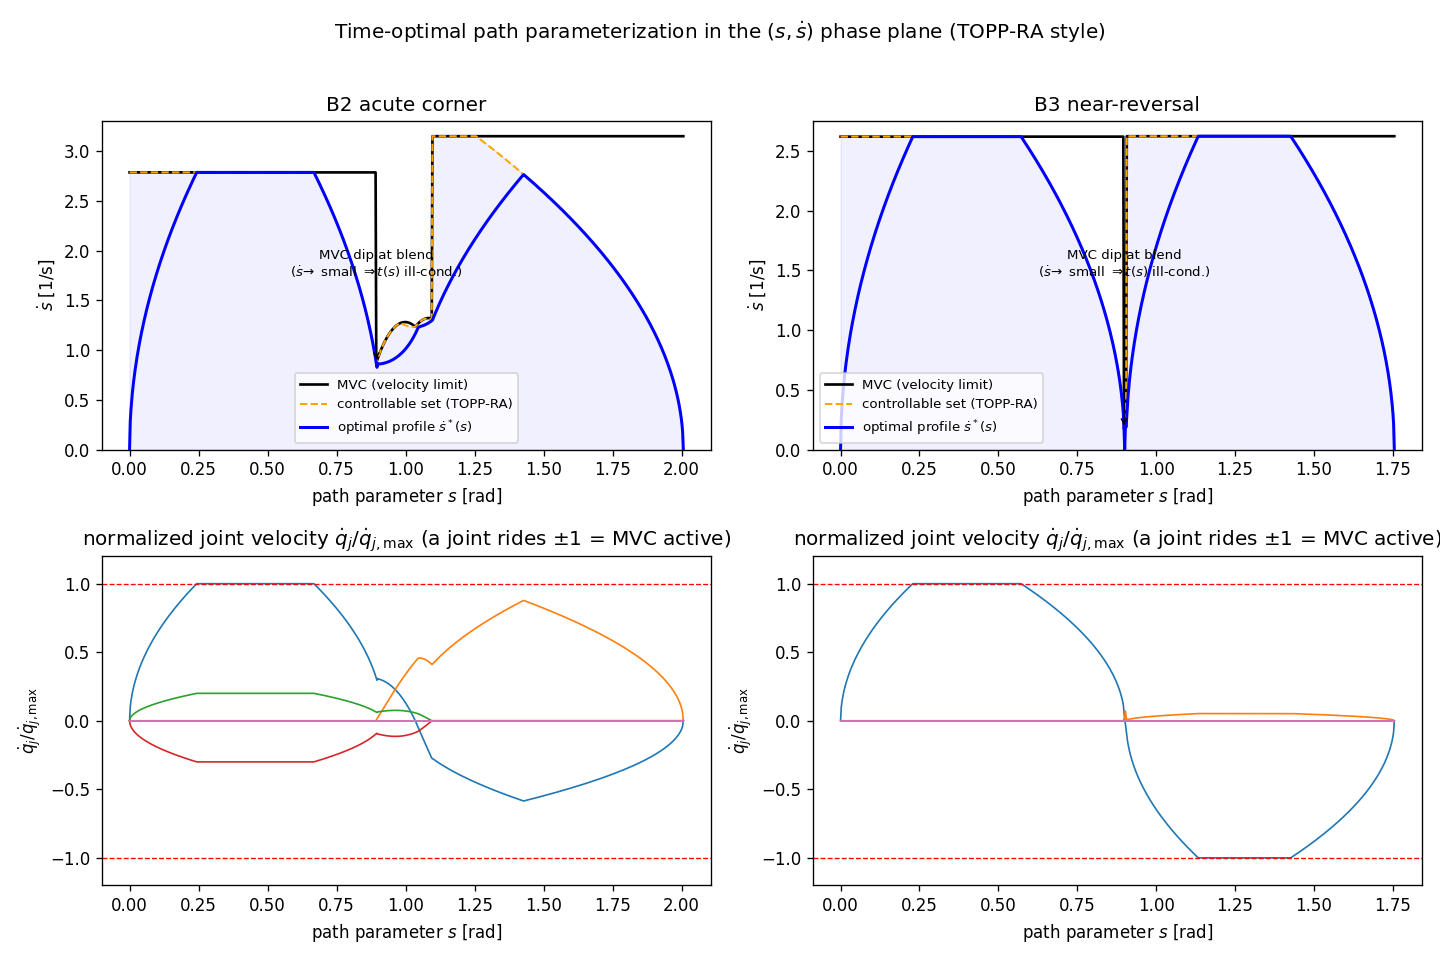
\includegraphics[keepaspectratio,alt={Phase-plane figure}]{benchmarks/topp_phaseplane.png}}
\emph{\textbf{Figure 1.} Time-optimal path parameterization in the
\((s,\dot s)\) phase plane (TOPP-RA style). The optimal profile dips at
the tight blend and---on the near-reversal---plunges to
\(\dot s\approx 0\), exactly where the \(s\!\to\!t\) map becomes
singular.}

\subsubsection{B. FR3 Manipulator
Results}\label{b.-fr3-manipulator-results}

Stresses are concentrated in two joints for interpretability while all
seven are planned. The decisive metric is the peak acceleration ratio
\(\lVert\ddot q\rVert_\infty/\ddot q_{\max}\): a value above \(1\) means
the emitted trajectory violates the declared acceleration limit. The DI
planner enforces this as a hard QP constraint and is pinned at \(1.000\)
with zero violations in every scenario.

{\def\LTcaptype{none} % do not increment counter
\begin{longtable}[]{@{}
  >{\raggedright\arraybackslash}p{(\linewidth - 14\tabcolsep) * \real{0.1250}}
  >{\raggedright\arraybackslash}p{(\linewidth - 14\tabcolsep) * \real{0.1250}}
  >{\raggedright\arraybackslash}p{(\linewidth - 14\tabcolsep) * \real{0.1250}}
  >{\raggedright\arraybackslash}p{(\linewidth - 14\tabcolsep) * \real{0.1250}}
  >{\raggedright\arraybackslash}p{(\linewidth - 14\tabcolsep) * \real{0.1250}}
  >{\raggedright\arraybackslash}p{(\linewidth - 14\tabcolsep) * \real{0.1250}}
  >{\raggedright\arraybackslash}p{(\linewidth - 14\tabcolsep) * \real{0.1250}}
  >{\raggedright\arraybackslash}p{(\linewidth - 14\tabcolsep) * \real{0.1250}}@{}}
\toprule\noalign{}
\begin{minipage}[b]{\linewidth}\raggedright
Scenario
\end{minipage} & \begin{minipage}[b]{\linewidth}\raggedright
DI \(T\) {[}s{]}
\end{minipage} & \begin{minipage}[b]{\linewidth}\raggedright
TOTG \(T\) {[}s{]}
\end{minipage} & \begin{minipage}[b]{\linewidth}\raggedright
DI accel ratio
\end{minipage} & \begin{minipage}[b]{\linewidth}\raggedright
TOTG accel ratio
\end{minipage} & \begin{minipage}[b]{\linewidth}\raggedright
TOTG accel viol.
\end{minipage} & \begin{minipage}[b]{\linewidth}\raggedright
DI jerk RMS
\end{minipage} & \begin{minipage}[b]{\linewidth}\raggedright
TOTG jerk RMS
\end{minipage} \\
\midrule\noalign{}
\endhead
\bottomrule\noalign{}
\endlastfoot
B1 point-to-point & 2.02 & \textbf{0.59} & 1.000 & 1.000 & 0 &
\textbf{22} & 143 \\
B2 acute corner (tight blend) & 1.92 & \textbf{1.23} & 1.000 &
\textbf{1.047} & 2 & 36 & 133 \\
B3 near-reversal & 1.99 & 1.07 & 1.000 & up to \textbf{3.13} & 1--4 & 29
& 166 \\
B4 dense (24 waypoints) & 13.24 & \textbf{3.83} & 1.000 & \textbf{1.445}
& 49 & \textbf{54} & 333 \\
\end{longtable}
}

\textbf{Timing table.} To avoid confusion between decoupled and coupled
cases (measurements from the accompanying single-threaded Python
harness, OSQP with absolute/relative tolerance \(10^{-6}\) in the
current scripts, warm-starting enabled, and KKT sparsity fixed for the
coupled obstacle update path):

{\def\LTcaptype{none} % do not increment counter
\begin{longtable}[]{@{}
  >{\raggedright\arraybackslash}p{(\linewidth - 6\tabcolsep) * \real{0.2500}}
  >{\raggedright\arraybackslash}p{(\linewidth - 6\tabcolsep) * \real{0.2500}}
  >{\raggedright\arraybackslash}p{(\linewidth - 6\tabcolsep) * \real{0.2500}}
  >{\raggedright\arraybackslash}p{(\linewidth - 6\tabcolsep) * \real{0.2500}}@{}}
\toprule\noalign{}
\begin{minipage}[b]{\linewidth}\raggedright
Case
\end{minipage} & \begin{minipage}[b]{\linewidth}\raggedright
Variables
\end{minipage} & \begin{minipage}[b]{\linewidth}\raggedright
Mean solve {[}ms{]}
\end{minipage} & \begin{minipage}[b]{\linewidth}\raggedright
Worst-case solve {[}ms{]}
\end{minipage} \\
\midrule\noalign{}
\endhead
\bottomrule\noalign{}
\endlastfoot
Decoupled box constraints (7 DOF, N=20) & 140 & 0.05--0.09 &
\textasciitilde0.4 \\
Coupled obstacle QP (Method A, fixed-sparsity update) & 141 & 2.1 &
9.8 \\
Decoupled goal reaction (warm-started) & 140 & 0.03 & --- \\
\end{longtable}
}

\textbf{Horizon sweep.} The same harness was swept over
\(N=\{10,20,30,40\}\) on the FR3 dynamic-obstacle problem using the
fixed-sparsity coupled QP (\texttt{sweep\_N.py}). The obstacle scenario
uses a velocity-law/APF reference, so completion time and clearance are
not very sensitive to \(N\) in this particular test; the dominant trend
is computational.

{\def\LTcaptype{none} % do not increment counter
\begin{longtable}[]{@{}
  >{\raggedleft\arraybackslash}p{(\linewidth - 12\tabcolsep) * \real{0.1429}}
  >{\raggedleft\arraybackslash}p{(\linewidth - 12\tabcolsep) * \real{0.1429}}
  >{\raggedleft\arraybackslash}p{(\linewidth - 12\tabcolsep) * \real{0.1429}}
  >{\raggedleft\arraybackslash}p{(\linewidth - 12\tabcolsep) * \real{0.1429}}
  >{\raggedleft\arraybackslash}p{(\linewidth - 12\tabcolsep) * \real{0.1429}}
  >{\raggedleft\arraybackslash}p{(\linewidth - 12\tabcolsep) * \real{0.1429}}
  >{\raggedleft\arraybackslash}p{(\linewidth - 12\tabcolsep) * \real{0.1429}}@{}}
\toprule\noalign{}
\begin{minipage}[b]{\linewidth}\raggedleft
Horizon \(N\)
\end{minipage} & \begin{minipage}[b]{\linewidth}\raggedleft
Look-ahead {[}s{]}
\end{minipage} & \begin{minipage}[b]{\linewidth}\raggedleft
Completion {[}s{]}
\end{minipage} & \begin{minipage}[b]{\linewidth}\raggedleft
Min EE clearance {[}m{]}
\end{minipage} & \begin{minipage}[b]{\linewidth}\raggedleft
Jerk RMS {[}rad/s³{]}
\end{minipage} & \begin{minipage}[b]{\linewidth}\raggedleft
Solve p95 {[}ms{]}
\end{minipage} & \begin{minipage}[b]{\linewidth}\raggedleft
Full cycle p95 {[}ms{]}
\end{minipage} \\
\midrule\noalign{}
\endhead
\bottomrule\noalign{}
\endlastfoot
10 & 0.10 & 1.86 & 0.297 & 275.5 & 1.09 & 2.55 \\
20 & 0.20 & 1.83 & 0.296 & 277.3 & 4.45 & 6.12 \\
30 & 0.30 & 1.84 & 0.298 & 292.7 & 20.85 & 23.04 \\
40 & 0.40 & 1.86 & 0.296 & 289.2 & 56.90 & 59.40 \\
\end{longtable}
}

The static waypoint sweep in the same script shows why \(N=20\) remains
the default: \(N=10\) can inflate time-to-goal dramatically for pure
position-tracking waypoints, while \(N\geq30\) increases coupled-QP
latency without improving clearance in the dynamic-obstacle test.

\textbf{Comparison scope.} The acceleration violation metric compares
the trajectory as emitted by each planner---i.e., the command sequence
as-sent to the controller, with no downstream smoothing or
re-interpolation applied to either planner's output. In practice, some
systems apply a final spline pass to the TOTG output before execution,
which would reduce or eliminate the resampling-induced violations on B2
and B4; under such post-processing the DI planner's zero-violation
advantage on those scenarios shrinks. The advantage on B3 (near-reversal
singularity) and in the reactive scenarios (Sections VI.D--F) is
independent of downstream smoothing.

Figure 2 plots the acceleration ratio over time for each scenario: the
DI curve never crosses \(1\), while the TOTG curve spikes above it at
blend seams.

\pandocbounded{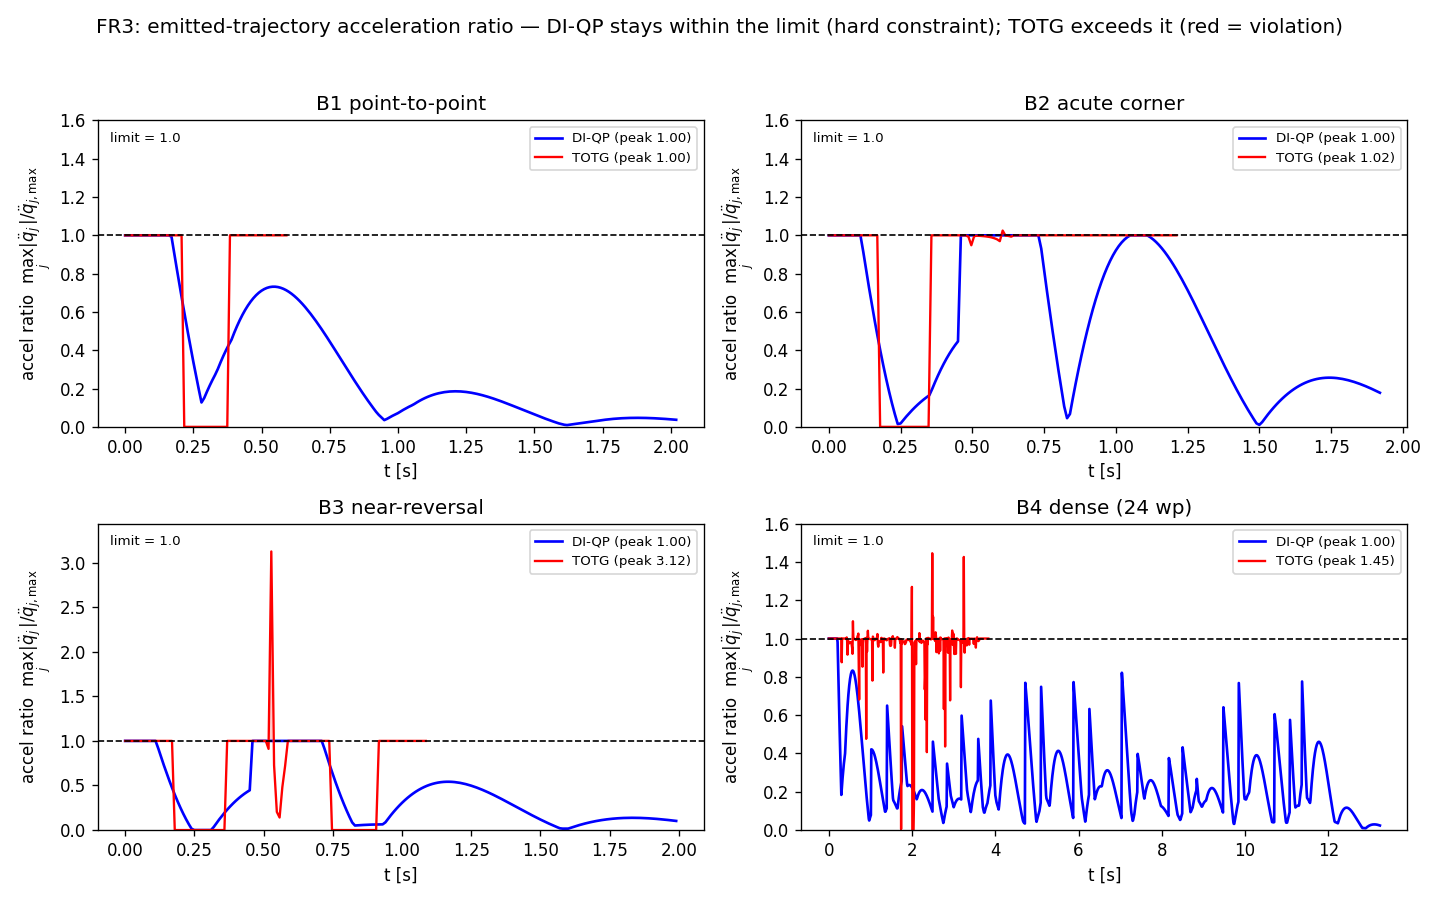
\includegraphics[keepaspectratio,alt={FR3 acceleration-ratio comparison}]{benchmarks/fr3_accel_compare.png}}
\emph{\textbf{Figure 2.} FR3 emitted-trajectory acceleration ratio
\(\max_j|\ddot q_j|/\ddot q_{j,\max}\) over time, DI-QP (blue) vs TOTG
(red), for B1--B4. The dashed line is the limit (\(=1\)). DI-QP is
pinned within the limit by its hard constraints; TOTG exceeds it at
blend seams---slightly on the corner (B2, \(1.047\times\)), dramatically
on the near-reversal (B3, up to \(3.13\times\)), and repeatedly on the
dense path (B4, \(1.445\times\)).}

In \textbf{B3 (near-reversal)} the blend radius collapses,
\(\dot s\to 0\), and the parameterization becomes singular:
\(\max(1/\dot s)\to\infty\) and the \(s\!\to\!t\) conversion fails
(flagged and capped by the harness). In \textbf{B4} the path-first
command breaks the acceleration limit by 45\% at 49 samples. The DI
planner remains feasible and smooth throughout.

\textbf{Robustness to the parameterizer (TOPP-RA).} To rule out a
weak-baseline artifact, we re-ran with reachability-based
\textbf{TOPP-RA} {[}7{]}---the modern parameterizer designed to be
robust at dynamic singularities. The structural findings persist: at the
acute corner the resampled command still exceeds the acceleration limit
(\(1.020\times\) under TOPP-RA versus \(1.047\times\) for the
numerical-integration baseline used in the main FR3 table); on the dense
path it still violates (\(1.12\times\) at 33 samples); and the
near-reversal remains singular (\(\min\dot s = 0\)) for both
parameterizers. TOPP-RA does soften magnitudes---the dramatic
\(3.13\times\) B3 spike drops to \(1.000\times\) under TOPP-RA---pinning
down what is implementation-dependent (spike size) versus intrinsic to
path-first (the violation itself from the curvature-discontinuous
reconstruction, and the \(\dot s\to0\) singularity). Note that replacing
the circular-arc blends with a \(C^2\) spline removes the acceleration
violations on B2 and B4 entirely; this confirms the violations arise
from the blend geometry, and that TOPP-RA on a \(C^2\) path is a
competitive baseline the DI planner cannot claim strict superiority over
on those metrics.

\textbf{Time-optimality.} TOTG is the lower bound by construction, and
the quadratic-cost DI planner pays for its smoothness in time (B1
\(3.4\times\), B4 \(3.5\times\) slower). Supplying the analytic
time-optimal velocity-law reference recovers the gap to
\(1.06\)--\(1.32\times\) while the DI-QP still preserves zero limit
violations. Thus the DI planner remains feasible by construction with
respect to the declared time-domain bounds, while path-first feasibility
can be lost after circular-blend reconstruction and uniform-time
resampling unless a smoother path representation or downstream
post-processing is used.

\subsubsection{C. Autonomous Vehicle Motion Planning with the
Double-Integrator
Backbone}\label{c.-autonomous-vehicle-motion-planning-with-the-double-integrator-backbone}

The same architectural principle extends naturally to autonomous-vehicle
motion planning. As with the manipulator case, the objective of the
planner is not to compute actuator commands directly, but rather to
generate a feasible time-parameterized trajectory that satisfies
kinematic constraints while remaining responsive to changing
environmental conditions.

Production autonomous-driving stacks such as Apollo separate planning
from control. The planner produces a sequence of trajectory points
containing position, heading, curvature, speed, and acceleration
information, while downstream lateral and longitudinal controllers
generate steering, throttle, and braking commands required to track the
trajectory. The planner output therefore takes the form

\[
\mathcal T = \{ x(t), y(t),\theta(t),\kappa(t),v(t),a(t) \},
\]

which is analogous to the manipulator trajectory

\[ \mathcal T = \left \{ q_d(t), \dot q_d(t), \ddot q_d(t) \right \}. \]

\paragraph{Vehicle Kinematic Model}\label{vehicle-kinematic-model}

Consider the standard kinematic bicycle model

\[ \dot x = v \cos\theta, \]

\[ \dot y = v \sin\theta, \]

\[\dot\theta = \frac{v}{L}\tan\delta,\]

\[ \dot v = a, \]

where \(L\) is the wheelbase, \(\delta\) is the steering angle, and
\(a\) is the longitudinal acceleration.

The governing equations of the vehicle remain these nonlinear kinematic
relationships. However, as in the manipulator formulation, a virtual
Cartesian double-integrator planning parameterization can be used as a
time-domain trajectory generator. This does not by itself remove vehicle
feasibility constraints; it produces candidate Cartesian position,
velocity, and acceleration profiles from which heading, curvature,
steering, and acceleration limits must be checked or constrained. The
resulting planning coordinates evolve as a virtual double-integrator
system,

\[ \ddot p = u, \]

where

\[ p = \begin{bmatrix} x\\ y \end{bmatrix},
u = \begin{bmatrix} u_x \\ u_y \end{bmatrix}\]

are virtual planning accelerations.

Defining the planning state

\[ X = \begin{bmatrix} p\\ \dot p \end{bmatrix},\]

the resulting prediction model becomes

\[ \dot X = \begin{bmatrix} 0&I\\ 0&0\end{bmatrix} X + \begin{bmatrix} 0\\ I \end{bmatrix} u. \]

This is identical to the double-integrator backbone used for manipulator
planning and therefore inherits the same constant state-transition
matrix (A\_d), offline prediction-matrix construction, and
fixed-structure QP formulation. The vehicle-specific feasibility
conditions enter through additional algebraic constraints or post-checks
on the recovered quantities, rather than through a
configuration-dependent prediction matrix.

\paragraph{Trajectory Generation}\label{trajectory-generation}

The planner directly optimizes a trajectory in the time domain rather
than constructing a geometric path followed by a separate
time-parameterization stage. Position, velocity, and acceleration
profiles are generated simultaneously within a single receding-horizon
optimization.

At each cycle, the optimizer produces a horizon of predicted Cartesian
states

\[ \{x(k),y(k),\dot x(k),\dot y(k),\ddot x(k),\ddot y(k)\} _{k=1}^{N},\]

from which heading and curvature are recovered through the vehicle
kinematics,

\[ \theta(k)=\operatorname{atan2}(\dot y(k),\dot x(k)),\]

\[ \kappa(k) = \frac{\dot x(k)\ddot y(k)-\dot y(k)\ddot x(k)}
{\left(\dot x(k)^2+\dot y(k)^2\right)^{3/2}}. \]

Curvature is computed only when \(v=\sqrt{\dot x^2+\dot y^2}>v_{\min}\);
below this threshold the previous curvature estimate is retained.
Feasibility with respect to the bicycle model requires, at minimum,

\[|\kappa(k)| \leq \kappa_{\max}=\frac{\tan\delta_{\max}}{L},\]

\[v(k)^2|\kappa(k)| \leq a_{y,\max},\]

and bounds on speed and longitudinal acceleration. These constraints can
be appended to the QP only after linearization, or enforced as
acceptance checks followed by replanning. The final planner output is
therefore a standard autonomous-driving trajectory consisting of

\[ (x,y,\theta,\kappa,v,a) \]

sampled at discrete time intervals.

\paragraph{Separation of Planning and
Control}\label{separation-of-planning-and-control}

The planner does not generate steering or throttle commands directly.
Instead, steering angle, throttle, and braking commands are computed by
downstream tracking controllers using the planned trajectory as
reference.

Consequently, the autonomous-vehicle formulation follows the same
planning/control separation as the manipulator formulation:

\[ \text{Vehicle Feasibility Checks / Linearized Constraints} \rightarrow
\text{Double-Integrator Trajectory Backbone} \rightarrow
\text{Predictive Motion Planner} \rightarrow
(x,y,\theta,\kappa,v,a) \]

followed by

\[ (x,y,\theta,\kappa,v,a) \rightarrow (\delta, T,B)\]

within the control layer.

This preserves a unified interpretation of the proposed framework: the
double-integrator backbone is a configuration-independent planning model
used to generate candidate trajectories, while vehicle-specific
feasibility and execution remain the responsibility of added constraints
and a separate control system.

\paragraph{AV Steering Benchmark}\label{av-steering-benchmark}

The accompanying AV harness evaluates the steering quantities recovered
from the planned Cartesian trajectory. This benchmark is diagnostic: a
pure Cartesian double-integrator trajectory can still exceed
steering-rate limits if curvature is not constrained. To show the effect
of adding the missing steering-rate smoothness, the harness also
includes a jerk-bounded lateral extension (a triple-integrator lateral
backbone) at fixed cruise speed. This extension is not the main
double-integrator contribution, but it illustrates the same time-domain
principle: optimize the derivative that must be bounded, then recover
vehicle commands from the resulting trajectory.

{\def\LTcaptype{none} % do not increment counter
\begin{longtable}[]{@{}
  >{\raggedright\arraybackslash}p{(\linewidth - 10\tabcolsep) * \real{0.1364}}
  >{\raggedright\arraybackslash}p{(\linewidth - 10\tabcolsep) * \real{0.1364}}
  >{\raggedleft\arraybackslash}p{(\linewidth - 10\tabcolsep) * \real{0.1818}}
  >{\raggedleft\arraybackslash}p{(\linewidth - 10\tabcolsep) * \real{0.1818}}
  >{\raggedleft\arraybackslash}p{(\linewidth - 10\tabcolsep) * \real{0.1818}}
  >{\raggedleft\arraybackslash}p{(\linewidth - 10\tabcolsep) * \real{0.1818}}@{}}
\toprule\noalign{}
\begin{minipage}[b]{\linewidth}\raggedright
Scenario
\end{minipage} & \begin{minipage}[b]{\linewidth}\raggedright
Planner
\end{minipage} & \begin{minipage}[b]{\linewidth}\raggedleft
Peak steering {[}deg{]}
\end{minipage} & \begin{minipage}[b]{\linewidth}\raggedleft
Peak steering rate {[}rad/s{]}
\end{minipage} & \begin{minipage}[b]{\linewidth}\raggedleft
Steering jump {[}rad{]}
\end{minipage} & \begin{minipage}[b]{\linewidth}\raggedleft
Peak lateral accel {[}m/s²{]}
\end{minipage} \\
\midrule\noalign{}
\endhead
\bottomrule\noalign{}
\endlastfoot
Single lane change & jerk-bounded time-first & 3.6 & \textbf{0.129} &
\textbf{0.0065} & 3.99 \\
Single lane change & TOTG path-first & 1.5 & 0.254 & 0.0254 & 2.47 \\
Double lane change & jerk-bounded time-first & 3.6 & \textbf{0.129} &
\textbf{0.0065} & 4.00 \\
Double lane change & TOTG path-first & 3.4 & 0.594 & 0.0594 & 4.05 \\
\end{longtable}
}

With a representative steering-rate cap of 0.5 rad/s, the jerk-bounded
time-first planner stays within the actuator-rate envelope in both
cruise maneuvers, whereas the path-first command exceeds the cap on the
double lane change because circular-blend curvature steps at path seams.
The pure Cartesian double-integrator variant, also reported by the
harness, is intentionally not claimed to satisfy steering-rate
constraints without adding curvature/rate constraints or a higher-order
lateral state.

\subsubsection{D. Bounded-Latency Reactive
Replanning}\label{d.-bounded-latency-reactive-replanning}

The reactivity advantage is structural rather than
implementation-dependent. A planar point robot must reach a goal while a
disk obstacle crosses its straight-line path mid-execution. The DI
planner recomputes an APF velocity reference from the obstacle's current
position each 100 Hz cycle and re-solves the box-constrained QP,
deflecting continuously. The path-first planner must halt, rebuild a
detour path, and re-run TOPP from rest.

Both reach the goal collision-free, but with very different cost
structure. The DI planner's \textbf{worst reaction latency is \(0.71\)
ms and is independent of the scene}: it is a single fixed-size QP. We
sweep the replan latency from \(0\) to \(400\) ms:

{\def\LTcaptype{none} % do not increment counter
\begin{longtable}[]{@{}
  >{\raggedright\arraybackslash}p{(\linewidth - 6\tabcolsep) * \real{0.2500}}
  >{\raggedright\arraybackslash}p{(\linewidth - 6\tabcolsep) * \real{0.2500}}
  >{\raggedright\arraybackslash}p{(\linewidth - 6\tabcolsep) * \real{0.2500}}
  >{\raggedright\arraybackslash}p{(\linewidth - 6\tabcolsep) * \real{0.2500}}@{}}
\toprule\noalign{}
\begin{minipage}[b]{\linewidth}\raggedright
Added path-search latency
\end{minipage} & \begin{minipage}[b]{\linewidth}\raggedright
TOTG completion {[}s{]}
\end{minipage} & \begin{minipage}[b]{\linewidth}\raggedright
TOTG time halted {[}s{]}
\end{minipage} & \begin{minipage}[b]{\linewidth}\raggedright
DI completion {[}s{]}
\end{minipage} \\
\midrule\noalign{}
\endhead
\bottomrule\noalign{}
\endlastfoot
0 (TOPP only) & 6.28 & 0.08 & \textbf{6.53 (flat)} \\
100 ms & 6.35 & 0.36 & 6.53 \\
200 ms & 6.63 & 0.66 & 6.53 \\
400 ms & 7.18 & 1.26 & 6.53 \\
\end{longtable}
}

The structural advantage is bounded by a fixed optimization structure
whose size grows with the number of active obstacle constraints: DI
deflects within one cycle and never halts, whereas TOTG must stop and
rebuild. The reactive edge is decisive when replanning is expensive
(full geometric search) or obstacles are fast, and marginal when the
rebuild is cheap. The DI planner does not demonstrate lower total
throughput; with zero replan latency, TOTG and DI have comparable
completion times.

\pandocbounded{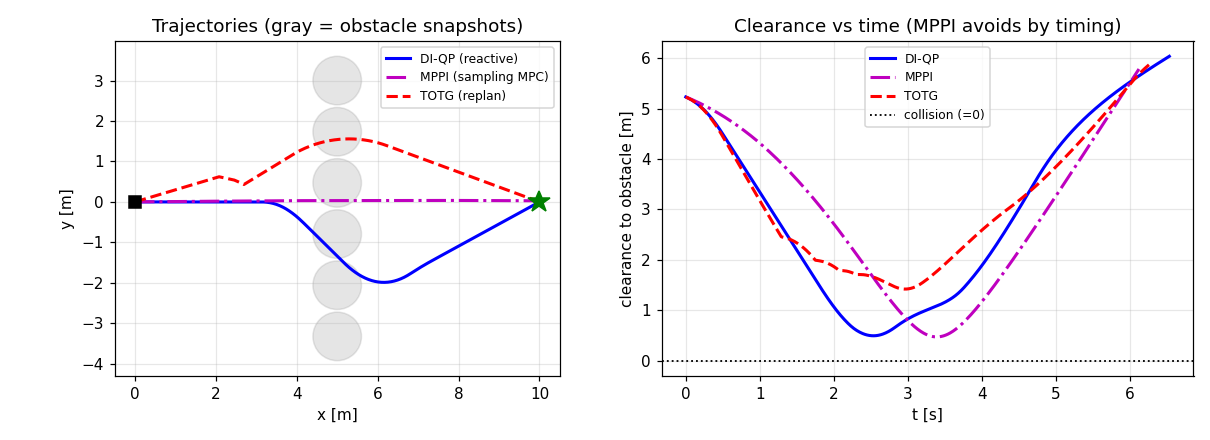
\includegraphics[keepaspectratio,alt={Dynamic obstacle, planar}]{benchmarks/dynamic_obstacle.png}}
\emph{\textbf{Figure 4.} Planar dynamic-obstacle test: the DI planner
(solid) deflects continuously; the path-first planner (dashed) halts and
rebuilds. DI reaction latency is bounded at \(0.71\) ms independent of
scene complexity.}

\subsubsection{E. APF Local-Minimum Failure and Waypoint-Injection
Recovery}\label{e.-apf-local-minimum-failure-and-waypoint-injection-recovery}

The APF method is intentionally presented as a soft, high-throughput
heuristic rather than a collision-certificate method. To expose its
failure mode, we place a planar double-integrator robot, goal, and
circular obstacle on the same line. With a purely radial APF field, the
attractive and repulsive terms balance in front of the obstacle and the
planner stalls. A simple waypoint-injection rule detects lack of
progress and inserts a lateral detour sequence around the obstacle; the
same box-constrained QP then reaches the goal while preserving velocity
and acceleration bounds (\texttt{apf\_local\_minimum.py}).

{\def\LTcaptype{none} % do not increment counter
\begin{longtable}[]{@{}lrr@{}}
\toprule\noalign{}
Metric & Pure APF & Waypoint injection \\
\midrule\noalign{}
\endhead
\bottomrule\noalign{}
\endlastfoot
Reached goal & no & yes \\
Completion / final time {[}s{]} & 17.99 & 15.56 \\
Final distance to goal {[}m{]} & 6.07 & 0.12 \\
Min obstacle clearance {[}m{]} & 0.22 & 0.22 \\
Max speed {[}m/s{]} & 1.50 & 1.50 \\
Max acceleration {[}m/s²{]} & 3.00 & 3.00 \\
Mean QP solve {[}ms{]} & 0.092 & 0.135 \\
\end{longtable}
}

This benchmark motivates the hybrid recommendation used throughout the
paper: APF reference deflection is useful for fast reactive steering,
but hard polytope constraints or explicit waypoint/safe-corridor logic
should be activated when progress stalls or clearance must be certified.

\subsubsection{F. Scaling to the 7-DOF Arm with a Dynamic
Obstacle}\label{f.-scaling-to-the-7-dof-arm-with-a-dynamic-obstacle}

We exercise the full Section IV machinery on the 7-DOF FR3, where
obstacle constraints couple the joints through the translational
Jacobian. The arm reaches a joint-space goal while a spherical obstacle
crosses the end-effector path. We compare against a
resolved-rate-plus-APF reactive controller without hard limits.

{\def\LTcaptype{none} % do not increment counter
\begin{longtable}[]{@{}lll@{}}
\toprule\noalign{}
Metric & DI-QP & Reactive baseline \\
\midrule\noalign{}
\endhead
\bottomrule\noalign{}
\endlastfoot
Reached goal & yes & yes \\
Min EE clearance {[}m{]} & 0.296 & 0.339 \\
Joint velocity violations & \textbf{0} & 42 \\
Joint acceleration violations & \textbf{0} & 346 \\
Worst-case solve {[}ms{]} & 9.8 & --- \\
Max slack used {[}m{]} & 0.000 & --- \\
\end{longtable}
}

Both avoid the obstacle and reach the goal. The reactive
baseline---lacking hard constraints---exceeds the joint velocity limit
at 42 samples and the acceleration limit at 346, whereas the QP holds
every joint limit exactly (zero violations) and keeps the linearized
half-space feasible throughout (zero slack). Replacing the original
rebuild-per-cycle prototype with a fixed-sparsity OSQP update path
reduces the nominal coupled-QP solve timing to 2.1 ms mean, 4.4 ms p95,
and 9.8 ms worst case on the harness
(\texttt{fixed\_sparsity\_timing.py}). Including Python-side assembly
and update overhead, the full per-cycle timing is 3.8 ms mean, 6.1 ms
p95, and 11.7 ms worst case; thus this Python harness meets 100 Hz at
p95, while worst-case cycles exceed 10 ms without further implementation
optimization.

\pandocbounded{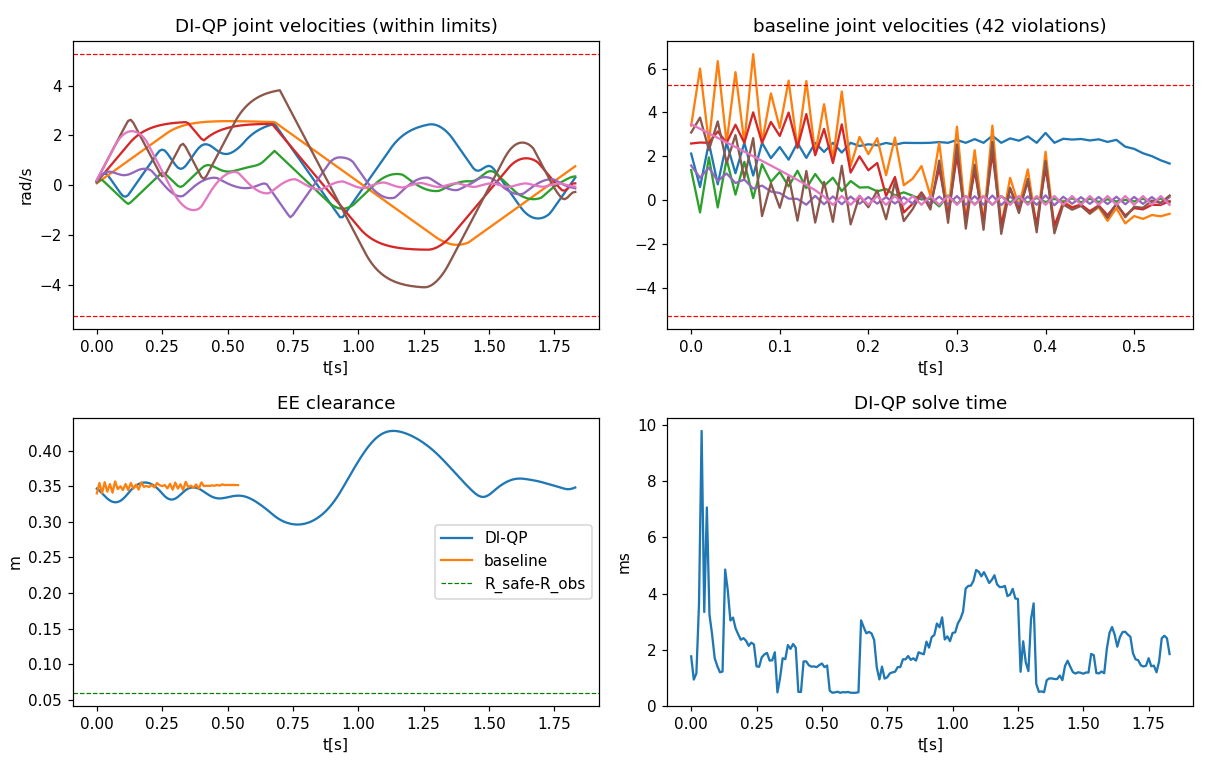
\includegraphics[keepaspectratio,alt={FR3 dynamic-obstacle signals}]{benchmarks/fr3_dynamic.png}}
\emph{\textbf{Figure 5.} 7-DOF FR3 dynamic obstacle. Top-left: DI-QP
joint velocities, all within the limit. Top-right: resolved-rate+APF
baseline, which exceeds the velocity limit. Bottom-left: end-effector
clearance. Bottom-right: DI-QP per-cycle solve time.}

\pandocbounded{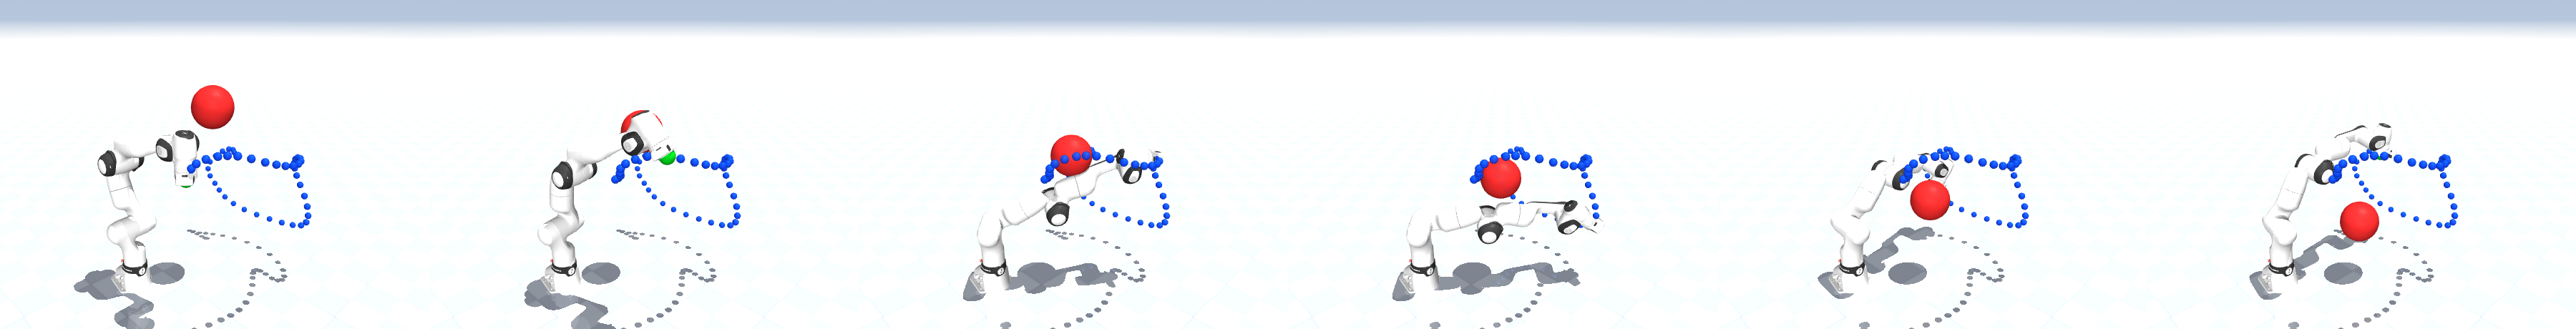
\includegraphics[keepaspectratio,alt={FR3 obstacle-avoidance render}]{benchmarks/fr3_motion.png}}
\emph{\textbf{Figure 6.} MuJoCo render of the FR3 executing the planned
trajectory while the spherical obstacle (red) descends through the
workspace.}

\subsubsection{G. Randomized FR3 Dynamic-Obstacle
Robustness}\label{g.-randomized-fr3-dynamic-obstacle-robustness}

To check that the dynamic-obstacle result is not tied to a single
hand-picked configuration, we perturb the start and goal joint states,
obstacle lateral offset, initial height, and crossing speed over 20
randomized trials (\texttt{fr3\_dynamic\_randomized.py}, seed 7). Both
planners reach the goal in all trials and avoid the obstacle. The
distinction is constraint fidelity: the QP maintains hard joint limits
in every trial, while the resolved-rate baseline repeatedly exceeds
them.

{\def\LTcaptype{none} % do not increment counter
\begin{longtable}[]{@{}lrr@{}}
\toprule\noalign{}
Metric & DI-QP & Reactive baseline \\
\midrule\noalign{}
\endhead
\bottomrule\noalign{}
\endlastfoot
Success rate & 100\% & 100\% \\
Min EE clearance, mean ± std {[}m{]} & 0.293 ± 0.018 & 0.328 ± 0.021 \\
Worst min EE clearance {[}m{]} & 0.261 & 0.266 \\
Total joint velocity violations & \textbf{0} & 618 \\
Total joint acceleration violations & \textbf{0} & 6889 \\
Max slack used {[}m{]} & 0.0000 & --- \\
QP solve p95 / max {[}ms{]} & ≈5.3 / ≈13.6 & --- \\
\end{longtable}
}

The baseline tends to keep slightly larger clearance because it is
unconstrained and can command arbitrarily aggressive joint velocities
and accelerations. The QP accepts a smaller but still positive clearance
while preserving every declared joint limit.

\subsubsection{H. Physical Execution in
MuJoCo}\label{h.-physical-execution-in-mujoco}

To verify that planner-level differences survive contact with rigid-body
dynamics, we execute both references on a torque-controlled FR3 in
MuJoCo (3.8.1; full mass matrix and gravity). A \(500\) Hz
computed-torque controller tracks each \(100\) Hz reference on the
acute-corner maneuver.

{\def\LTcaptype{none} % do not increment counter
\begin{longtable}[]{@{}lll@{}}
\toprule\noalign{}
Metric (joint 1 / worst) & DI-QP & TOTG \\
\midrule\noalign{}
\endhead
\bottomrule\noalign{}
\endlastfoot
Peak demanded torque {[}Nm{]} & 58.0 & 56.7 \\
Torque-rate RMS {[}Nm/s{]} & \textbf{181} & 383 \\
Samples over torque limit & 0 & 0 \\
Tracking RMSE {[}mrad{]} & 1.9 & 2.0 \\
\end{longtable}
}

Both stay within the torque envelope and track to \(\approx 2\) mrad
RMS. TOTG's acceleration discontinuity at the blend seam manifests
physically as a stepped torque command (torque-rate RMS \(2.1\times\)
that of the DI reference), while the DI reference produces a smooth
torque profile. TOTG completes the fixed path faster; the DI command is
gentler on the drivetrain. This visualizes the smoothness-versus-time
trade-off in closed-loop physics rather than at the planner output.

\pandocbounded{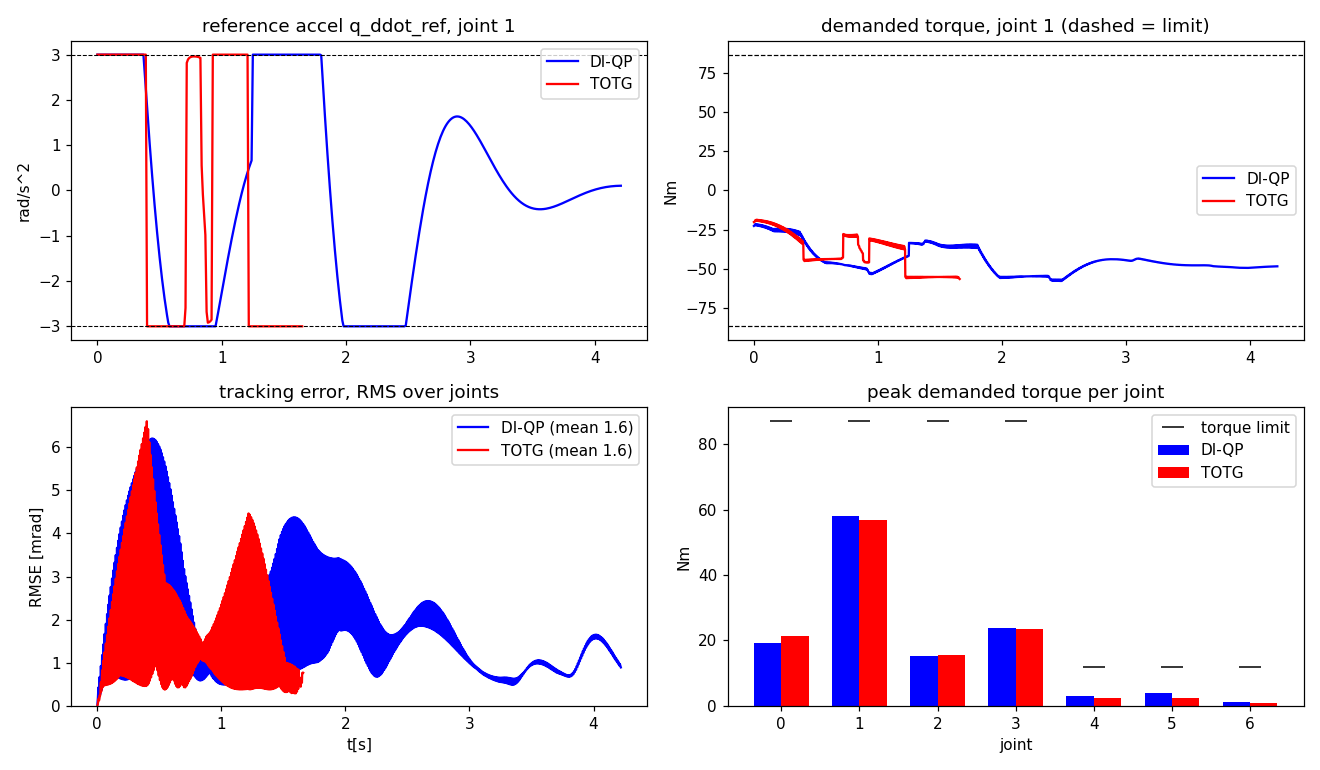
\includegraphics[keepaspectratio,alt={MuJoCo computed-torque comparison}]{benchmarks/mujoco_compare.png}}
\emph{\textbf{Figure 7.} FR3 computed-torque execution in MuJoCo. DI
reference produces smooth acceleration and torque; TOTG produces stepped
commands at blend seams. Both remain within torque limits. Tracking RMSE
is comparable.}

\begin{center}\rule{0.5\linewidth}{0.5pt}\end{center}

\subsection{VII. Implementation Notes}\label{vii.-implementation-notes}

\subsubsection{A. Solver Configuration}\label{a.-solver-configuration}

The QP is solved with OSQP {[}4{]} using the following configuration:

\begin{itemize}
\tightlist
\item
  \textbf{Warm-starting:} The previous solution \(U^*\) is used as the
  initial point for the next solve, reducing cold-start latency from
  \textasciitilde5 ms to under 0.5 ms for the decoupled box-constrained
  QPs in the benchmark harness.
\item
  \textbf{Sparse structure exploitation:} The Hessian \(H\) is assembled
  once offline. In the decoupled benchmark, the OSQP object is set up
  once and only vectors are updated online. In the coupled-obstacle
  benchmark, the obstacle half-space uses a fixed sparsity pattern and
  updates numeric values in place via OSQP's \texttt{Ax} update; this
  avoids rebuilding the symbolic factorization each cycle.
\item
  \textbf{Horizon length:} At a \(100\) Hz planning rate
  (\(\Delta t = 10\) ms), \(N = 10\) (0.1 s look-ahead) is too short for
  pure position-tracking waypoint tasks---time-to-goal can inflate by
  several times. The \textbf{recommended default is \(N = 20\) (\(0.2\)
  s)}: it recovers most achievable speed in the decoupled waypoint
  benchmarks while keeping the fixed-sparsity coupled obstacle QP within
  a few milliseconds p95 solve time. Increasing to \(N \approx 30\) can
  narrow the static time-optimality gap in some cases, but it increases
  jerk and, for coupled obstacle constraints, raises solve time
  substantially.
\end{itemize}

\subsubsection{B. Goal Sequencing and Waypoint
Tracking}\label{b.-goal-sequencing-and-waypoint-tracking}

For multi-waypoint tasks, the goal state \(x_{\text{goal}}\) is updated
online as waypoints are reached (within a threshold \(\epsilon_q\)).
Because the planner is formulated in the time domain with a receding
horizon, waypoint transitions are smooth and require no explicit path
splicing or re-initialization.

\subsubsection{C. Computational
Complexity}\label{c.-computational-complexity}

For \(n\) joints and horizon \(N\), the decision variable count is
\(nN\). For a 7-DOF robot with \(N = 20\), this yields 140 decision
variables in the box-constrained case and 141 variables when a single
shared obstacle slack is added. OSQP, warm-started, converges in well
under a millisecond for decoupled box-constrained QPs and in a few
milliseconds for the fixed-sparsity coupled obstacle QP on commodity
CPUs. Coupled obstacle constraints increase both the row count and the
cost of sparse linear algebra, but the symbolic structure can remain
fixed while only numeric values change. The precomputed \(\Phi\) and
\(\Gamma\) matrices are formed once at initialization and never rebuilt;
the online computational burden is dominated by the QP solve itself
(ADMM iterations and sparse linear solves inside OSQP), not by
prediction-matrix construction, which has been entirely eliminated
through offline precomputation. This is the practical computational
benefit of the constant-\(A_d\) property.

\begin{center}\rule{0.5\linewidth}{0.5pt}\end{center}

\subsection{VIII. Discussion}\label{viii.-discussion}

The proposed framework achieves a specific, well-defined shift in the
motion planning architecture: rather than planning in space and then
parameterizing in time, trajectory generation and time-domain constraint
enforcement are unified in a single, continuously-running optimization
loop. The constant-\(A_d\) property---derived from the nilpotency of the
double-integrator system matrix---is the enabling structural insight. It
decouples the computational burden of trajectory prediction from robot
configuration, making real-time replanning at 100 Hz viable on standard
hardware.

\subsubsection{Scope and Limitations}\label{scope-and-limitations}

This framework should be understood as a \textbf{local predictive motion
planner} rather than a complete global planner. Several limitations
bound the current formulation:

\textbf{(i) Not time-optimal by default.} With a pure position-tracking
cost the planner regulates to the goal like a damped second-order
system, easing off before using full actuator authority, inflating
time-to-goal to \(3\)--\(3.5\times\) TOTG. This is largely recoverable
by supplying the analytic time-optimal velocity-law reference, which
closes the gap to \(1.06\)--\(1.32\times\) while preserving zero limit
violations. The velocity reference can thus be viewed as a tunable
speed-versus-smoothness selector. The table below summarizes the
trade-off across the main operating points and recommends application
domains:

{\def\LTcaptype{none} % do not increment counter
\begin{longtable}[]{@{}
  >{\raggedright\arraybackslash}p{(\linewidth - 10\tabcolsep) * \real{0.1667}}
  >{\raggedright\arraybackslash}p{(\linewidth - 10\tabcolsep) * \real{0.1667}}
  >{\raggedright\arraybackslash}p{(\linewidth - 10\tabcolsep) * \real{0.1667}}
  >{\raggedright\arraybackslash}p{(\linewidth - 10\tabcolsep) * \real{0.1667}}
  >{\raggedright\arraybackslash}p{(\linewidth - 10\tabcolsep) * \real{0.1667}}
  >{\raggedright\arraybackslash}p{(\linewidth - 10\tabcolsep) * \real{0.1667}}@{}}
\toprule\noalign{}
\begin{minipage}[b]{\linewidth}\raggedright
Mode
\end{minipage} & \begin{minipage}[b]{\linewidth}\raggedright
\(R\) (accel. weight)
\end{minipage} & \begin{minipage}[b]{\linewidth}\raggedright
Velocity reference
\end{minipage} & \begin{minipage}[b]{\linewidth}\raggedright
Time vs.~TOTG
\end{minipage} & \begin{minipage}[b]{\linewidth}\raggedright
Jerk RMS
\end{minipage} & \begin{minipage}[b]{\linewidth}\raggedright
Recommended for
\end{minipage} \\
\midrule\noalign{}
\endhead
\bottomrule\noalign{}
\endlastfoot
Maximum smoothness & large (\(\geq 1.0\)) & position-tracking only &
\(3\)--\(3.5\times\) & low (\textasciitilde22) & Human collaboration,
compliant tasks \\
Balanced & medium (\(0.1\)) & position-tracking only &
\(2\)--\(2.5\times\) & medium & General manipulation \\
Near-time-optimal & small (\(0.01\)) & analytic velocity law &
\(1.06\)--\(1.32\times\) & high (\textasciitilde bang-bang) &
High-throughput assembly, no humans \\
\end{longtable}
}

The near-time-optimal mode approaches bang-bang acceleration, which is
acceptable when downstream actuators tolerate rapid torque changes; the
smoothness mode is preferable whenever human proximity or drivetrain
longevity is a concern.

\textbf{(ii) Linearization accuracy.} Jacobian linearization (Method A)
is accurate only in a neighborhood of the current configuration; its
error grows roughly quadratically in joint-speed × horizon. In the FR3
harness, the end-horizon error is already about 10 cm at 50\% joint
speed over a 0.2 s horizon. For fast motions or large obstacles
requiring significant detours, the horizon should be shortened, the
safety margin inflated using a Hessian/remainder bound, or the accepted
rollout checked against the nonlinear geometry.

\textbf{(iii) Local minima.} APF-based avoidance (Method B) is
susceptible to local minima in complex environments. Persistent
feasibility under the finite QP horizon can be improved by appending a
terminal safe set (e.g., a maximal-braking-to-rest profile) at the end
of the horizon.

\textbf{(iv) Finite look-ahead.} The \(N = 20\) horizon at 100 Hz
provides \(0.2\) s look-ahead, which may be insufficient for very
fast-moving obstacles.

\subsubsection{Relationship to Path-First and Path--Velocity
Pipelines}\label{relationship-to-path-first-and-pathvelocity-pipelines}

The path-first baseline (TOTG, TOPP-RA) is time-optimal by construction
and plans the entire path at once, providing advantages the proposed
planner does not match on static tasks. The acceleration violations on
B2 and B4 arise from circular-blend geometry rather than from time
parameterization itself; replacing circular arcs with a \(C^2\) spline
removes them entirely. Similarly, the near-reversal singularity is
mitigated once the path carries bounded curvature. These observations
motivate using a high-quality path representation with any time
parameterizer.

What remains intrinsic to the path-first structure, and unrepairable
without architectural change, is: (a) the absence of bounded per-cycle
reactivity---any change triggers a full batch rebuild; and (b) the
requirement for a precomputed geometric path. These are precisely the
limitations the proposed time-domain architecture addresses. The two
approaches are complementary: the proposed planner trades global
time-optimality and full-path lookahead for feasibility, smoothness,
conditioning at geometric degeneracies, and bounded-latency reactivity.

Many industrial motion-planning systems employ a two-stage architecture
that separates geometric path generation from temporal trajectory
generation. Examples include autonomous-driving systems such as Apollo
and manipulator frameworks such as MoveIt. The proposed framework should
be read against that background: it borrows the virtual-integrator
planning philosophy used in speed planning, but removes the fixed-path
assumption by optimizing the configuration trajectory directly.

\paragraph{Autonomous Driving: Apollo Planning
Architecture}\label{autonomous-driving-apollo-planning-architecture}

Apollo employs a hierarchical planning architecture consisting of a
path-planning stage followed by a speed-planning stage {[}11{]}. The
path planner first generates a collision-free geometric path
parameterized by arc length \(s\), \(x(s),y(s)\), while satisfying lane
boundaries and obstacle constraints. A subsequent speed optimizer
computes the temporal evolution \(s(t)\), subject to velocity,
acceleration, jerk, and dynamic-obstacle constraints.

The speed-planning stage is commonly formulated using a virtual
double-integrator model, \(\ddot{s}=u\), where the optimization variable
is the path acceleration. This abstraction decouples trajectory
generation from the full nonlinear vehicle dynamics and enables
efficient real-time optimization.

The proposed framework follows a similar philosophy. Rather than
planning directly with the nonlinear manipulator dynamics, trajectory
generation is performed in a virtual joint-space model, \(\ddot{q}=u\).
However, unlike Apollo, which optimizes only the timing along a
previously fixed path, the proposed method directly optimizes the entire
joint-space trajectory. Path generation, timing, and obstacle avoidance
are therefore solved simultaneously within a single convex optimization
problem.

\paragraph{Manipulator Planning: MoveIt and Time
Parameterization}\label{manipulator-planning-moveit-and-time-parameterization}

A similar decomposition appears in many industrial manipulator planning
pipelines. For example, MoveIt typically generates a collision-free
geometric path using a sampling-based planner such as OMPL and
subsequently applies a time-parameterization algorithm such as Iterative
Parabolic Time Parameterization (IPTP) or Time-Optimal Trajectory
Generation (TOTG). The resulting pipeline can be summarized as

\[\text{Path Planning} \rightarrow
\text{Time Parameterization} \rightarrow
\text{Trajectory Execution}. \]

Collision avoidance is therefore addressed during path generation,
whereas velocity and acceleration limits are enforced afterward during
time parameterization. In contrast, the proposed formulation directly
optimizes \(q(t)\) over the prediction horizon while simultaneously
enforcing joint limits, velocity limits, acceleration limits, and
workspace obstacle constraints. This removes the need for a separate
time-parameterization stage and enables reactive replanning when
obstacles or task objectives change.

\paragraph{Comparison with Trajectory Optimization and
MPC}\label{comparison-with-trajectory-optimization-and-mpc}

Methods such as CHOMP, TrajOpt, and nonlinear Model Predictive Control
also optimize complete trajectories directly. However, these methods
generally employ nonlinear robot models and repeatedly recompute
Jacobians, Hessians, or linearized state-transition matrices during
optimization.

The key distinction of the proposed approach is the use of a
configuration-independent virtual double-integrator model. Because the
system matrices are constant,

\[
A_c= \begin{bmatrix}
0&I\\ 0&0
\end{bmatrix},
\]

the discrete prediction matrices \(\Phi\) and \(\Gamma\) can be computed
offline and reused for all planning cycles. Consequently, the online
optimization involves only the solution of a convex quadratic program
with fixed prediction structure.

\paragraph{Positioning of the Proposed
Method}\label{positioning-of-the-proposed-method}

The proposed framework may be interpreted as extending the
virtual-integrator planning philosophy used in autonomous-driving speed
planners to high-dimensional manipulator motion planning. Unlike
traditional path-then-time approaches, the proposed method directly
optimizes the joint-space trajectory while incorporating obstacle
avoidance and kinematic constraints into a unified predictive
optimization problem. Compared with nonlinear trajectory optimization
and dynamic MPC formulations, the approach sacrifices explicit dynamic
modeling in exchange for a fixed prediction structure, lower
computational complexity, and high-rate replanning capability. The
primary contribution is therefore not the introduction of a new dynamic
model, but rather the use of a configuration-independent virtual
double-integrator planning model that enables offline computation of
prediction matrices and efficient online trajectory optimization for
multi-degree-of-freedom manipulators.

\subsubsection{Validation Gaps}\label{validation-gaps}

Three gaps bound the present evidence. First, validation is
simulation-only; a physical FR3 demonstration with a moving
obstacle---showing that the claimed reactivity holds on real hardware
without safety stops---is the most important next experimental step.
Second, the comparison covers path-first methods and a
resolved-rate-plus-APF reactive baseline. The dynamic obstacle test
(Section VI.D) compares against a full-stop-and-rebuild TOTG pipeline; a
stronger baseline would be an incremental geometric replanner (e.g.,
RRT* or OMPL with a warm-start from the previous path) paired with
TOPP-RA, which would reduce replan latency and narrow the reactivity
gap. Such a comparison is deferred to future work, but is explicitly
needed to support the reactivity claim against state-of-the-art online
replanning methods. A head-to-head comparison against nonlinear MPC,
differential dynamic programming, MPPI, or learned reactive policies
would further situate the method in the broader landscape. Third, only
the FR3 dynamic-obstacle experiment currently includes a randomized
robustness study; the remaining tables are single-scenario or small
scenario-suite evaluations. Future work should report means and standard
deviations over at least 20--50 randomized trials per benchmark family
to establish robustness claims that are not sensitive to the specific
configurations chosen.

\begin{center}\rule{0.5\linewidth}{0.5pt}\end{center}

\subsection{IX. Conclusion}\label{ix.-conclusion}

This paper presented a unified time-domain local Predictive Motion
Planner built on a constant state-transition double-integrator backbone.
The central observation---that a virtual double-integrator planner
yields a constant \(A_d\) independent of robot configuration---enables
offline precomputation of all dynamics prediction matrices, reducing
online computation to a convex QP with bounded per-cycle latency for a
fixed active constraint structure. The resulting planner produces
\(C^1\) trajectories \((q_d, \dot{q}_d, \ddot{q}_d)\) with hard-bounded
acceleration and reacts to workspace changes through receding-horizon QP
updates, achieving a form of bounded reactive behavior that is
structurally unavailable to batch plan-then-execute pipelines. For
applications requiring continuous acceleration, the same construction
extends to a piecewise-jerk triple-integrator backbone with constant
prediction matrices. The framework was inspired by the pHRI
architecture, but employs the resulting double-integrator backbone
solely as a planning model, independent of any particular low-level
cancellation strategy.

Future work will validate the framework on a physical 7-DOF manipulator,
extend obstacle avoidance to non-convex environments via safe-corridor
decomposition, and benchmark against online MPC and trajectory
optimization methods.

\begin{center}\rule{0.5\linewidth}{0.5pt}\end{center}

\subsection{References}\label{references}

{[}1{]} I. A. Şucan, M. Moll, and L. E. Kavraki, ``The Open Motion
Planning Library,'' \emph{IEEE Robot. Autom. Mag.}, vol.~19, no. 4,
pp.~72--82, 2012.

{[}2{]} D. Lertkultanon and Q.-C. Pham, ``Time-optimal path
parameterization for redundantly actuated robots,'' \emph{IEEE/ASME
Trans. Mechatronics}, vol.~21, no. 4, pp.~1643--1651, 2016.

{[}3{]} Anonymous Author(s), ``Impedance MPC for Physical Human--Robot
Interaction: Predictive Disturbance Rejection with Joint-Limit Safety,''
\emph{submitted for review}, 2024.

{[}4{]} B. Stellato, G. Banjac, P. Goulart, A. Bemporad, and S. Boyd,
``OSQP: An operator splitting solver for quadratic programs,''
\emph{Math. Program. Comput.}, vol.~12, no. 4, pp.~637--672, 2020.

{[}5{]} S. Liu \emph{et al.}, ``Planning dynamically feasible
trajectories for quadrotors using safe flight corridors in 3-D complex
environments,'' \emph{IEEE Robot. Autom. Lett.}, vol.~2, no. 3,
pp.~1688--1695, 2017.

{[}6{]} O. Khatib, ``Real-time obstacle avoidance for manipulators and
mobile robots,'' \emph{Int. J. Robot. Res.}, vol.~5, no. 1, pp.~90--98,
1986.

{[}7{]} H. Pham and Q.-C. Pham, ``A new approach to time-optimal path
parameterization based on reachability analysis,'' \emph{IEEE Trans.
Robot.}, vol.~34, no. 3, pp.~645--659, 2018.

{[}8{]} O. Khatib, ``A unified approach for motion and force control of
robot manipulators: The operational space formulation,'' \emph{IEEE J.
Robot. Autom.}, vol.~3, no. 1, pp.~43--53, 1987.

{[}9{]} D. Q. Mayne \emph{et al.}, ``Constrained model predictive
control: Stability and optimality,'' \emph{Automatica}, vol.~36, no. 6,
pp.~789--814, 2000.

{[}10{]} T. Kunz and M. Stilman, ``Time-optimal trajectory generation
for path following with bounded acceleration and velocity,'' in
\emph{Robotics: Science and Systems}, 2012.

{[}11{]} ApolloAuto, ``Apollo: An open autonomous driving platform,''
GitHub repository, https://github.com/ApolloAuto/apollo, accessed June
17, 2026.

\section{Appendix A. Unconstrained ARE Solution of the Double-Integrator
Planning
Backbone}\label{appendix-a.-unconstrained-are-solution-of-the-double-integrator-planning-backbone}

This appendix illustrates the unconstrained LQR solution associated with
the double-integrator planning backbone. The result provides a useful
reference trajectory generator and clarifies the relationship between
the analytical Linear Quadratic Regulator (LQR) characterization and the
constrained predictive motion planner developed in the main text.

\subsection{A.1 Double-Integrator Planning
Model}\label{a.1-double-integrator-planning-model}

The planner employs the configuration-independent double-integrator
backbone

\[ \dot x = Ax + Bu,\]

with
\[ A= \begin{bmatrix} 0&I\\ 0&0\end{bmatrix}, \qquad B=\begin{bmatrix}0\\I\end{bmatrix},\]

where \(x=[q^\top, \dot q ^\top ]^\top\) contains the planned joint
positions and velocities, and \(u=\ddot q\) is the planned joint
acceleration. For a 7-DOF manipulator, \(q\in\mathbb{R}^7,
x\in\mathbb{R}^{14},
u\in\mathbb{R}^{7}.\) The planner output is the time-indexed trajectory
\(\mathcal T = \{q_d(t),\dot q_d(t),\ddot q_d(t)\}.\)

\subsection{A.2 Reference Generation from an End-Effector
Goal}\label{a.2-reference-generation-from-an-end-effector-goal}

Suppose the end effector is required to move from
\(p_0= [ 0, 0, 0 ]^\top\) to \(p_g=[ 1, 1, 1 ]^\top.\) Let \(p=f(q)\),
denote the forward kinematics. A desired joint-space target may be
obtained from inverse kinematics, \[q_g = IK(p_g), \]

or, locally, from the Jacobian linearization

\[q_g \approx q_0 + J(q_0)^\dagger \bigl(p_g-p_0\bigr). \]

The corresponding reference state is

\[x_r= \begin{bmatrix} q_g \\0 \end{bmatrix},\]

which represents the desired final configuration with zero velocity.

\subsection{A.3 Algebraic Riccati
Equation}\label{a.3-algebraic-riccati-equation}

For regulation to a nonzero reference, define the tracking error
\(e=x-x_r\). Consider the infinite-horizon quadratic cost

\[J = \int_0^\infty \left(e^\top Qe + u^\top Ru \right) dt,\]

where \(Q\succeq0, R\succ0.\) The continuous-time Algebraic Riccati
Equation is

\[A^\top P + PA - PBR^{-1}B^\top P + Q = 0.\]

The optimal feedback gain is \(K =R^{-1}B^\top P.\) For regulation to
the reference state, the optimal feedback law becomes \(u=-K(x-x_r).\)
Equivalently, \[ \ddot q = -K_p(q-q_g) - K_d\dot q,\]

where \(K_p\) and \(K_d\) are the position and velocity feedback
components contained within \(K\).

\subsection{A.4 Closed-Loop Trajectory
Generation}\label{a.4-closed-loop-trajectory-generation}

Define the tracking error \(e=x-x_r.\) Substituting the optimal control
law into the planning dynamics yields \(\dot e = (A-BK)e.\) Since the
closed-loop matrix \((A-BK)\) is Hurwitz, the tracking error converges
asymptotically to zero, \(e(t)\rightarrow0.\) The resulting joint
accelerations \(\ddot q(t)\) generate the velocity trajectory
\[\dot q(t) = \dot q(0) + \int_0^t \ddot q(\tau),d\tau,\]

and the position trajectory \[q(t) =q(0) +\int_0^t \dot q(\tau),d\tau.\]

Consequently, the ARE solution produces a complete trajectory
\[\mathcal T = \{q_d(t),\dot q_d(t),\ddot q_d(t)\}\]

that converges optimally toward the desired configuration.

\subsection{A.5 Feasibility Check}\label{a.5-feasibility-check}

The ARE solution represents the unconstrained optimum of the
double-integrator planning problem. The generated trajectory may
therefore be used as a candidate motion plan.

The trajectory is considered feasible if it satisfies all planning
constraints,

\[q_{\min} \le q_d(t) \le q_{\max},\]

\[|\dot q_d(t)| \le \dot q_{\max},\]

\[|\ddot q_d(t)| \le \ddot q_{\max},\]

and all workspace obstacle constraints. If these conditions are
satisfied, the ARE trajectory itself constitutes a valid motion plan.

If any constraint is violated, the unconstrained solution remains
optimal for the unconstrained problem but is no longer feasible for
motion planning. In this case, the constrained predictive planner
presented in the main text is invoked. The resulting MPC/QP formulation
can therefore be viewed as a finite-horizon constrained counterpart to
the unconstrained LQR/ARE solution, operating on the same
double-integrator backbone while explicitly enforcing kinematic and
environmental constraints.
